%% LyX 2.3.6.2 created this file.  For more info, see http://www.lyx.org/.
%% Do not edit unless you really know what you are doing.
\documentclass{article}
\usepackage{lmodern}
\usepackage{lmodern}
\usepackage[T1]{fontenc}
\usepackage[utf8]{inputenc}
\setcounter{secnumdepth}{-1}
\usepackage{amsmath}
\usepackage{amssymb}
\usepackage{graphicx}
\PassOptionsToPackage{normalem}{ulem}
\usepackage{ulem}
\usepackage{subscript}
\usepackage[unicode=true,
 bookmarks=false,
 breaklinks=false,pdfborder={0 0 1},backref=section,colorlinks=false]
 {hyperref}
\hypersetup{
 hidelinks,pdfcreator={LaTeX via pandoc}}

\makeatletter
%%%%%%%%%%%%%%%%%%%%%%%%%%%%%% Textclass specific LaTeX commands.
\newenvironment{lyxcode}
	{\par\begin{list}{}{
		\setlength{\rightmargin}{\leftmargin}
		\setlength{\listparindent}{0pt}% needed for AMS classes
		\raggedright
		\setlength{\itemsep}{0pt}
		\setlength{\parsep}{0pt}
		\normalfont\ttfamily}%
	 \item[]}
	{\end{list}}

\@ifundefined{date}{}{\date{}}
%%%%%%%%%%%%%%%%%%%%%%%%%%%%%% User specified LaTeX commands.
% Options for packages loaded elsewhere


%
\usepackage{iftex}
\ifPDFTeX
  \usepackage{textcomp}% provide euro and other symbols
\else % if luatex or xetex
  \usepackage{unicode-math}
\defaultfontfeatures{Scale=MatchLowercase}
  \defaultfontfeatures[\rmfamily]{Ligatures=TeX,Scale=1}
\fi
% Use upquote if available, for straight quotes in verbatim environments
\IfFileExists{upquote.sty}{\usepackage{upquote}}{}
\IfFileExists{microtype.sty}{% use microtype if available
  \usepackage[]{microtype}
  \UseMicrotypeSet[protrusion]{basicmath} % disable protrusion for tt fonts
}{}

\@ifundefined{KOMAClassName}{% if non-KOMA class
  \IfFileExists{parskip.sty}{%
    \usepackage{parskip}
  }{% else
    \setlength{\parindent}{0pt}
    \setlength{\parskip}{6pt plus 2pt minus 1pt}}
}{% if KOMA class
  \KOMAoptions{parskip=half}}

\usepackage{xcolor}
\IfFileExists{xurl.sty}{\usepackage{xurl}}{} % add URL line breaks if available
\IfFileExists{bookmark.sty}{\usepackage{bookmark}}{\usepackage{hyperref}}

\urlstyle{same} % disable monospaced font for URLs

\def\maxwidth{\ifdim\Gin@nat@width>\linewidth\linewidth\else\Gin@nat@width\fi}
\def\maxheight{\ifdim\Gin@nat@height>\textheight\textheight\else\Gin@nat@height\fi}

% Scale images if necessary, so that they will not overflow the page
% margins by default, and it is still possible to overwrite the defaults
% using explicit options in \includegraphics[width, height, ...]{}
\setkeys{Gin}{width=\maxwidth,height=\maxheight,keepaspectratio}
% Set default figure placement to htbp

\def\fps@figure{htbp}

\setlength{\emergencystretch}{3em} % prevent overfull lines
\providecommand{\tightlist}{%
  \setlength{\itemsep}{0pt}\setlength{\parskip}{0pt}}
 % remove section numbering
\ifLuaTeX
  \usepackage{selnolig}% disable illegal ligatures
\fi

\title{Exams (with answers) of module

Transient Groundwater Flow

from 2006 onwards\protect\hypertarget{_Toc91020611}{}{}}
\author{}

\makeatother

\begin{document}
\title{UNESCO-IHE}
\title{Exams Transient Groundwater FLow - from 2006-2022}
\title{With Answers}
\author{Prof. dr.ir. T.N.Olsthoorn}
\date{\emph{\today}}

\maketitle
\tableofcontents{}

\section{Open-book exam (1h), Feb 7, 2022}

\subsection{Question 1}

Questions 1.1 and 1.2

A well is installed at 250 m distance from a river. The well fully
penetrates the aquifer. The aquifer is unconfined, it has a conductivity
of k= 30~m/d and a representative thickness of 40~m, which may be
assumed constant. It further has a storage coefficient (specific yield)
of S=0.20. The well extracts water at a rate of \emph{Q}=1200~m\textsuperscript{3}/d
during exactly 7~days, after which it stops. The questions refer
to the drawdown in point p at 50 m from the well on the line through
the well perpendicular to the river as shown in the figure.

\begin{figure}
\begin{centering}
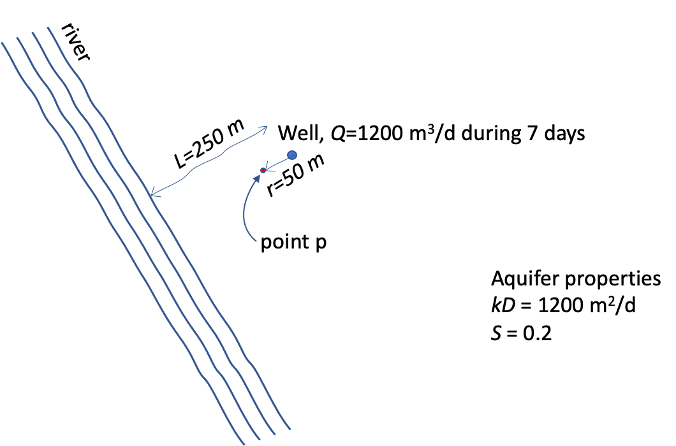
\includegraphics[width=0.8\textwidth]{pictures/2022_1}
\par\end{centering}
\caption{Well adjacent to a straight fully penetrating river. The aquifer is
homogeneous and extends to infinity.This is clearly a well in an aquifer
with constant transmissivity, for which the well-known Theis solution
is applicable. To obtain values for the Theis well function, you can
make use of the Theis type curve shown below.}
\end{figure}

\begin{figure}
\begin{centering}
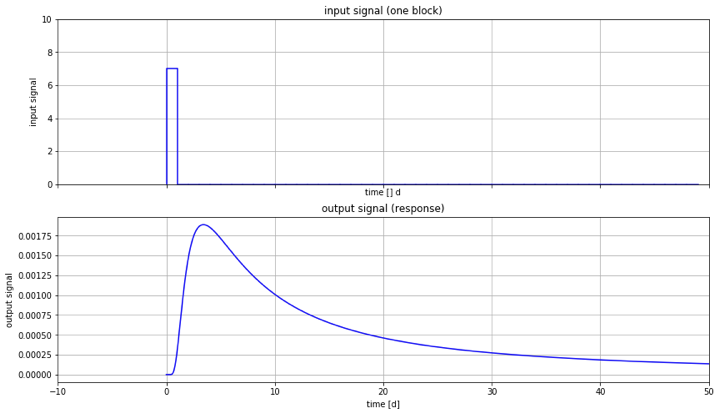
\includegraphics[width=0.8\textwidth]{pictures/2022_2}
\par\end{centering}
\caption{Theis type curve, i.e., the Theis well function as a function of $1/u$}
\end{figure}

\begin{enumerate}
\item What will be the drawdown at point p at $t=7$ d after the start of
the extraction? 
\end{enumerate}
\rule[0.5ex]{1\columnwidth}{1pt}

Generalities:

The transient drawdown due to a well in an aquifer of constant transmissivity
extracting at a constant rate from $t=0$ is according to the Theis
solution

\[
s(r,t)=\frac{Q}{4\pi\text{kD}}\mathrm{W}(u)\mbox{, with }u=\frac{r^{2}S}{4kDt}
\]

But we must take care of the river, which creates a fixed-head boundary
condition. This is done by placing a mirror well of opposite sign
at the exact opposite side of the river and at the same distance.
The formula for the well and its mirror well is

\[
s_{r,t}=\frac{Q}{4\pi kD}\left(\mathrm{W}\left(\frac{r_{1}^{2}S}{4kDt}\right)-\mathrm{W}\left(\frac{r_{2}^{2}S}{4kDt}\right)\right)
\]

In which $r_{1}=50$ m and $r_{2}=450$ m, $\text{kD}\ =\ 1200$ m2/d,
$S=0.2$

We also have $\frac{Q}{4\pi\text{kD}}=\frac{1200}{4\pi1200}=0.08$

Then for t=7 days

$u_{1}=1.49\times10^{-2}$, $u_{2}=1.21$,

$1\text{/}u_{1}=6.72\times10^{+1}$, $1\text{/}u_{2}=8.30\times10^{-1}$,
Then read the values for $W(1/u)$ from the Theis type graph, which
yields the following numbers (however yours may be a bit different
because it's difficult to read exact numbers from a graph.

$W\left(1.49\times10^{-2}\right)=3.6$, $W(1.21)=0.16$

So the drawdown after 7 days in point p is

$s_{t=7}=0.08\times(3.5-0.16)=0.28$ m

\rule[0.5ex]{1\columnwidth}{1pt}
\begin{enumerate}
\item What will be the drawdown at point p 14 days after the start of the
extraction, i.e. 7 days after the well has started pumping? 
\end{enumerate}
\rule[0.5ex]{1\columnwidth}{1pt}

For t = 14 days continuous pumping the values become

$u_{1}=7.44\times10^{-3}$, $u_{2}=6.03\times10^{-1}$,

$1\text{/}u_{1}=1.43\times10^{+2}$, $1\text{/}u_{2}=1.66$, read
the values of $\mathrm{W}(1/u)$ from the Theis type curve to get
the following values (which again may be a bit different from yours
due to the accuracy with which you can read the numbers from a graph):

$\mathrm{W}\left(7.44\times10^{-3}\right)=4.3$, $\mathrm{W}\left(6.03\times10^{-1}\right)=0.45$

Hence the drawdown for $t=14\,\mathrm{d}$ of continued pumping would
be

$s_{t=14}=0.08\times(4.30-0.45)=0.31\,\mathrm{m}$.

The actual drawdown after 14 days will be that of continuous pumpoing
(0.31 m) minus that of 7 days continuous pumping (0.28 m) because
the pump was switched off after 7 days. We, therefore, after 14 days
we only have a remaining drawdown equal to 0.31 -- 0.28 = 0.03 m.

\rule[0.5ex]{1\columnwidth}{1pt}

\subsection{Question 2}

The picture shows an aquifer bounded by a fully penetrating river
at \emph{x=0}. The aquifer is unbounded to the right and has a transmissivity
and a specific yield as indicated in the picture. Note that the transmissivity
may be considered constant. The river water level varies continuously
according to a sine-wave with a cycle time of \emph{T= 1} d and an
amplitude of \emph{A=1.2} m.

\begin{figure}
\begin{centering}
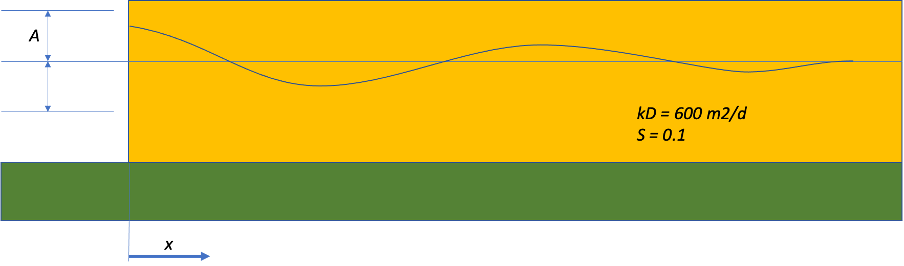
\includegraphics[width=0.8\textwidth]{pictures/2022_3}
\par\end{centering}
\caption{Aquifer bounded by fully penetrating water body with fluctuating water
level at x=0. The aquifer extents at the right to infinity. Shown
is the water table (or head) at an arbitrary time.}
\end{figure}

\begin{enumerate}
\item What is the maximum and minimum head at \emph{x = 25} m and at \emph{x
= 100} m? 
\item What will be the drawdown at point p 14 days after the start of the
extraction, i.e., 7 days after the well has started pumping? 
\item By how much (i.e., by how large a factor) does this delay change if
the storage coefficient would be 100 times as small as the given value,
i.e., if it would be $S=0.001$ instead of $S=0.1$? 
\end{enumerate}
\rule[0.5ex]{1\columnwidth}{1pt}

The formula for the head in this aquifer is

\[
s(x,t)=Ae^{-\text{ax}}\sin\left(\omega t-ax\right)
\]

With $a=\sqrt{\frac{\omega S}{2\text{kD}}}$, the damping factor and
$\omega T=2\pi\rightarrow\omega=\frac{2\pi}{T}$

The maximum and minimum head at any x is given by $s_{\max,\min}=\pm Ae^{-\text{ax}}$,
the so-called envelope.

$\omega=\frac{2\pi}{T}=\frac{2\pi}{1}=6.28$ radians/day

$a=\sqrt{\frac{\omega S}{2\text{kD}}}=\sqrt{\frac{6.28\times0.1}{2\times600}}=0.023$
{[}1/m{]}

At $x=25\,\mathrm{m}$, we have $s_{\min,\max}=\pm Ae^{-\text{ax}}=\pm1.2e^{-0.023\times25}=\pm0.68\,\mathrm{m}$.

At $x=100\,\mathrm{m}$, we have $s_{\min,\max}=\pm Ae^{-\text{ax}}=\pm1.2e^{-0.023\times100}=\pm0.12\,\mathrm{m}$.

What is the delay of the wave at \emph{x = 100} m relative to the
wave at \emph{x = 0} m?

The velocity of the wave follows from the argument of the sin being
constant

\[
\omega t-ax=\mathrm{const}
\]

Taking the derivative with respect to \emph{t} yields

\[
\omega-a\frac{dx}{dt}=0
\]

And so
\begin{quote}
$v=\frac{dx}{dt}=\frac{\omega}{a}=\frac{6.28}{0.023}\approx270\,\mathrm{m/d}$. 
\end{quote}
Hence, the delay at $x=100\,\mathrm{m}$ is $100\text{/}270=0.37\,\mathrm{d}\approx9\,\mathrm{h}$.

\rule[0.5ex]{1\columnwidth}{1pt}

\subsection{Question 3:}

The picture below shows an aquifer of limited lateral extent. To the
left, at \emph{x = 0}, it is bounded by a fully penetrating surface
water body, such as a lake. To the right, at \emph{x = L}, it is bounded
by an impervious land mass as shown. The aquifer properties are shown
in the picture, but you don't need them to answer the questions. The
water level of the lake and the groundwater table are initially flat
at a level equal to \emph{h=0}~m as indicated by the horizontal blue
line. At $t\ =\ 0$, the water level of the lake suddenly changes
upward by an amount \emph{A} as indicated. Ignore other hydrological
features like rain and evapotranspiration. Only the effect of the
sudden change of the lake level is considered.

\begin{figure}
\begin{centering}
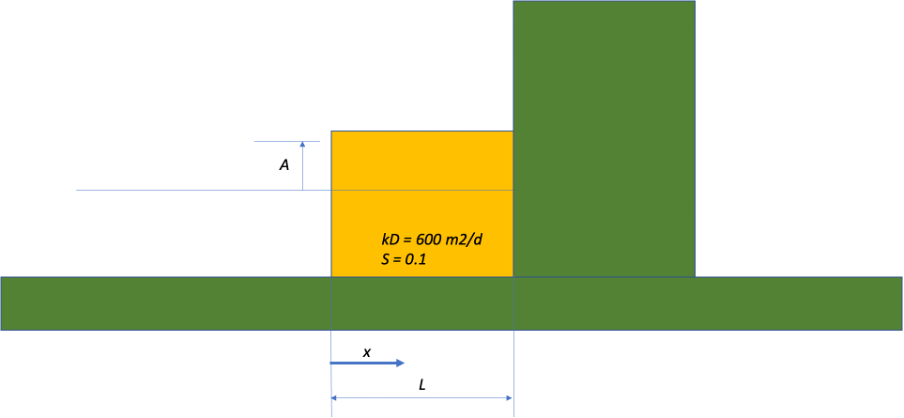
\includegraphics[width=0.8\textwidth]{pictures/2022_4}
\par\end{centering}
\caption{Picture of the aquifer with fully penetrating water body at $x=0$
and impervious mass at $x=L$}
\end{figure}

\begin{enumerate}
\item What are the boundary conditions at \emph{x=0} and \emph{x=L}? 
\end{enumerate}
\rule[0.5ex]{1\columnwidth}{1pt}

The boundary condtions are a) fixed head at $x=0$ and b) zero flow
at $x=L$.

\rule[0.5ex]{1\columnwidth}{1pt}
\begin{enumerate}
\item Describe how the head in the aquifer will develop over time due to
the sudden change at \emph{x=0} and \emph{t=0}. Your description must
include the situation at $t=0$ and at $t=\infty$.
\end{enumerate}
\rule[0.5ex]{1\columnwidth}{1pt}

At $t<0$, $s=0$ everywhere. At $t=0^{+}$, $s=A$ at $x=0$ and
$s=0$ everywhere else. At $t>0$, $s=A$ at $x=0$ and $A>s>0$ everywhere
else with $s_{x>x_{1}}<s_{x<x_{1}}$for arbitrary $x$ and, finally,
$s=A$ everywhere for $t=\infty$.

\rule[0.5ex]{1\columnwidth}{1pt}

\section{Closed-book exam (1h), Feb 23, 2021}

\subsection{Question 1}
\begin{enumerate}
\item When pumping from a confined aquifer, all extracted water comes from
storage. But what is the precise physical mechanism that causes the
release of water from this type of aquifer? Explain. 
\end{enumerate}
\rule[0.5ex]{1\columnwidth}{1pt}

Compression of the aquifer matrix and expansion of the water (combined
elastic response of the aquifer with its water)

\rule[0.5ex]{1\columnwidth}{1pt}
\begin{enumerate}
\item What is the so-called air-entry pressure and how does it relate to
the capillary fringe? Explain. 
\end{enumerate}
\rule[0.5ex]{1\columnwidth}{1pt}

This is the air pressure required to blow air through a sample of
initially saturated soil. It's a measure of the widest pores and coincides
with the thickness of the capillary zone.

\rule[0.5ex]{1\columnwidth}{1pt}
\begin{enumerate}
\item A confined aquifer system has a loading efficiency of LE = 0.6. If
the barometer pressure increases with the equivalent of 40 cm water
column, by how much does the pressure in the aquifer change? By how
much does the head (water level in a piezometer in this aquifer) change?
Explain and show. 
\end{enumerate}
\rule[0.5ex]{1\columnwidth}{1pt}

A loading efficiency of 60\% implies that 60 \% of the load at ground
surface will be supported by the water. Hence a loading at ground
surface by the barometer, which also exercises 100\% at the water
level in the piezometer will cause a decline of the head in the piezometer
by 40\% of the load, which, in this case is 40\% of 40 cm = 16 cm.

\rule[0.5ex]{1\columnwidth}{1pt}
\begin{enumerate}
\item What is the difference between a Theis and a Hantush situation? The
answer must contain the difference between the two situations as and
what the physical origin is of the water pumped from a well in both
these situations. 
\end{enumerate}
\rule[0.5ex]{1\columnwidth}{1pt}

In the Theis situation all extracted water is released from storage
and from storage only, while in the Hantush situation it also originates
from the leakage through a top or bottom aquitard induced by the drawdown.
The Theis drawdown, whether due to pumping a confined or an unconfined
aquifer will never reach equilibrium. However a Hantush drawdown will
reach equilibrium because the induced flow through the aquitard is
proportional to the local induced head difference and therefore will
eventually balance the extraction.

\rule[0.5ex]{1\columnwidth}{1pt}

\subsection{Question 2}

The solution for the head in a confined aquifer driven by surface
water that varies according to a sine at x=0 is given by

\[
h_{x,t}=Ae^{-ax}\sin\left(\omega t-ax\right)\text{, with }a=\sqrt{\frac{\omega}{2}\frac{S}{kD}}
\]

\begin{enumerate}
\item Explain what the parameters are with their dimension 
\end{enumerate}
\rule[0.5ex]{1\columnwidth}{1pt}

$h$ is dynamic head {[}m{]}, $A$ amplitude of river stage {[}m{]},
$a$ {[}1/m{]} damping factor, $\omega$ {[}rad/time{]} is angular
velocity of sine wave. $T$ {[}d{]} time, $x$ {[}m{]} distance from
the river, $S$ {[}-{]} storage coefficient either elastic or specific
yield, $kD\ \mathrm{m^{2}/d}$ transmissivity of the aquifer.

\rule[0.5ex]{1\columnwidth}{1pt}
\begin{enumerate}
\item What is the velocity of the wave in the subsurface? Explain mathematically. 
\end{enumerate}
\rule[0.5ex]{1\columnwidth}{1pt}

Take the argument of the sine as a constant hence $\omega t-ax=const$
and take the derivative with respect to time to get the velocity $\frac{dx}{dt}=v=\frac{\omega}{a}$

\rule[0.5ex]{1\columnwidth}{1pt}
\begin{enumerate}
\item What are the so-called envelopes? Explain and show them mathematically. 
\end{enumerate}
\rule[0.5ex]{1\columnwidth}{1pt}

The two envelopes show the maximum amplitude as a function of x, hence
$H_{x}=\pm e^{-ax}$

The dynamic change of head in a strip of land of limited width like
the one that is shown below can be computed using the simple formula
for a half-infinite aquifer, but then we must apply superposition
using so-called mirror ditches. In the figure below the water level
at the left-hand side has just jumped up by \emph{A} m and that at
the right-and side by \emph{B} m. The head for $t=0.29\,\mathrm{d}$
is shown. The lower picture shows the applied mirror/superposition
scheme.

\rule[0.5ex]{1\columnwidth}{1pt}

\subsection{Question 3:}

The dynamic change of head in a strip of land of limited width like
the one that is shown below can be computed using the simple formula
for a half-infinite aquifer, but then we must apply superposition
using so-called mirror ditches. In the figure below the water level
at the left-hand side has just jumped up by \emph{A} m and that at
the right-and side by \emph{B} m. The head for t=0.29 d is shown.
The lower picture shows the applied mirror/superposition scheme.
\begin{enumerate}
\item Is the shown mirror/superposition scheme used for the superposition
correct? Clearly motivate your answer, a simple yes or no is not accepted. 
\end{enumerate}
\rule[0.5ex]{1\columnwidth}{1pt}

The left and the right -hand boundaries are fixed. All errors to the
left and the right of the left-hand boundary cancel, so only the fixed
change at the left-hand boundary remains. This is ok. The same is
true for the right-hand boundary. Hence, the superposition schme is
correct.

\rule[0.5ex]{1\columnwidth}{1pt}

\begin{figure}
\begin{centering}
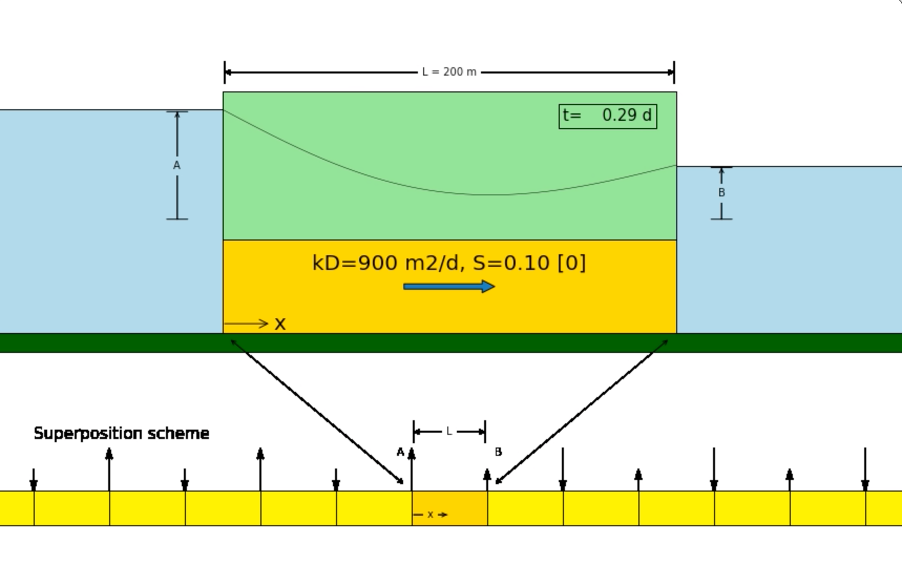
\includegraphics[width=0.8\textwidth]{pictures/2021_1}
\par\end{centering}
\caption{Strip of land bounded by fully penetrating surface water (top) and
superposition scheme (bottom).}
\end{figure}


\subsection{Question 4:}

During a pumping test with an extraction of $Q=650\,\mathrm{m^{3}/d}$,
the drawdown is measured in an observation well at $r=50\,\mathrm{m}$
distance from the well, sufficient to ignore any influence of partial
penetration on the measurements. The measured drawdown in this piezometer
is shown graphically versus the log of time in days.
\begin{figure}
\begin{centering}
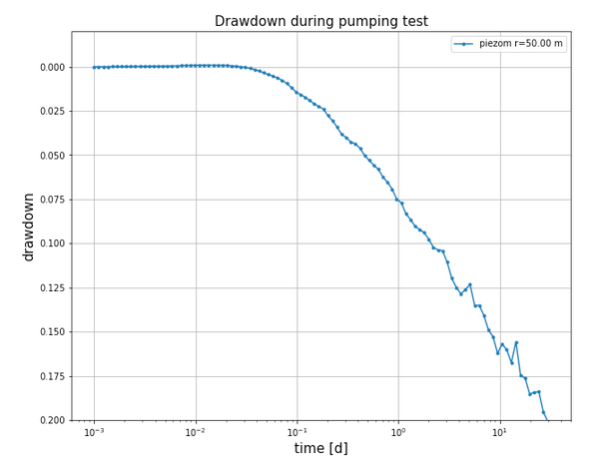
\includegraphics[width=0.8\textwidth]{pictures/2021_2}
\par\end{centering}
\caption{Measured drawdown during pumping test.}
\end{figure}

The formula for the drawdown that is expected to fit the data for
sufficiently large times is

\[
s_{r,t}\,=\,\frac{Q}{4\pi kD}\ln\left(\frac{2.25kDt}{r^{2}S}\right)
\]

\begin{enumerate}
\item Do these data represent a Theis (confined/unconfined) or a Hantush
(semi-confined) situation? Motivate your answer (a single yes or no
is not accepted). 
\end{enumerate}
\rule[0.5ex]{1\columnwidth}{1pt}

The curve represents a Theis drawdown, because there is no equilibrium.

\rule[0.5ex]{1\columnwidth}{1pt}
\begin{enumerate}
\item Determine the transmissivity of the aquifer 
\end{enumerate}
\rule[0.5ex]{1\columnwidth}{1pt}

We have:

\[
s_{r,t}=\frac{Q}{4\pi kD}\ln\left(\frac{2.25kDt}{r^{2}S}\right)=\frac{2.3\ Q}{4\pi kD}\log\left(\frac{2.25kDt}{r^{2}S}\right)
\]

With

$\Delta s_{r}=s_{r,10t}-s_{r,t}=\ \frac{2.3\ Q}{4\pi kD}\log\left(\frac{2.25kD10t}{r^{2}S}\right)-\frac{2.3\ Q}{4\pi kD}\log\left(\frac{2.25kD10t}{r^{2}S}\right)=\frac{2.3Q}{4\pi kD}\ \approx0.09\,\mathrm{m}$

It follows that

\[
0.09\approx\frac{2.3Q}{4\pi kD}\rightarrow kD\approx\frac{2.3Q}{4\pi0.09}=\frac{2.3\times650}{4\pi0.09}\approx1300\,\mathrm{m^{2}\text{/}d}
\]

\rule[0.5ex]{1\columnwidth}{1pt}
\begin{enumerate}
\item Determine the storage coefficient of the aquifer 
\end{enumerate}
\rule[0.5ex]{1\columnwidth}{1pt}

The storage coefficient can be computed from the zero drawdown in
the logarithmic approximation of the Theis drawdown, i.e., when the
argument of the log in the formula is one. This zero drawdown is at
about $t=0.1\,\mathrm{d}$, so $S=\frac{2.25kDt}{r^{2}}=\frac{2.25\times1300\times0.1}{2500}\approx0.1$

\rule[0.5ex]{1\columnwidth}{1pt}
\begin{enumerate}
\item What will be the radius of influence of this pumping test for \emph{t}
= 5 days? 
\end{enumerate}
\rule[0.5ex]{1\columnwidth}{1pt}

The radius of influence is $r=\sqrt{\frac{2.25kDt}{S}}=\sqrt{\frac{2.25\times1300\times5}{0.1}}\approx380$
$m$

\rule[0.5ex]{1\columnwidth}{1pt}

\section{Closed book exam (1h), Feb 4, 2020}

\subsection{Question 1}
\begin{enumerate}
\item Explain what is meant by air-entry pressure, and how you interpret
it in terms of groundwater. 
\end{enumerate}
\rule[0.5ex]{1\columnwidth}{1pt}

The air entry pressure is the pressure required to blow air through
a small soil sample. It corresponds to the suction head of the widest
pores, and, therefore, the thickness of the capillary fringe.

\rule[0.5ex]{1\columnwidth}{1pt}
\begin{enumerate}
\item What happens to the water level in a piezometer installed in a confined
aquifer if suddenly a load equivalent to a pressure increase $\Delta p$
is placed on ground surface? 
\end{enumerate}
\rule[0.5ex]{1\columnwidth}{1pt}

The water pressure increases by \emph{$LE$} times $\Delta p$. And
the head in the piezometer goes up by $\Delta\phi=LE\frac{\Delta p}{\rho g}$.

\rule[0.5ex]{1\columnwidth}{1pt}
\begin{enumerate}
\item What happens to the water level in a piezometer if the barometer pressure
suddenly change by an amount $\Delta p$? 
\end{enumerate}
\rule[0.5ex]{1\columnwidth}{1pt}

The water level would go up like answered in the previous question,
but because of the full barometer pressure pushing down on the water
level in the piezometer, it actually goes down by $\Delta\phi=BE\frac{\Delta p}{\rho g}=\left(1-LE\right)\frac{\Delta p}{\rho f}$.

\rule[0.5ex]{1\columnwidth}{1pt}
\begin{enumerate}
\item Explain what causes the difference between the answers to questions
2. And 3. 
\end{enumerate}
\rule[0.5ex]{1\columnwidth}{1pt}

It's already explained above.

\rule[0.5ex]{1\columnwidth}{1pt}
\begin{enumerate}
\item If a pressure transducer is fixed in a piezometer, below the water
level at a given elevation, then what changes would it register in
the two situations described in questions 2 and 3? (A pressure transducer
measures and registers the absolute pressure, i.e. water + air). 
\end{enumerate}
\rule[0.5ex]{1\columnwidth}{1pt}

A pressure transducer measuring absolute pressure will experience
a pressure increases of $\Delta p$ in both cases.

\rule[0.5ex]{1\columnwidth}{1pt}

\subsection{Question 2}

Let the time-dependent change of head in a strip of land with width
\emph{\ensuremath{L}} {[}m{]} between two ditches be caused by a sudden
change of water level equal to \emph{\ensuremath{A}} {[}m{]} at the
left ditch and equal to \emph{\ensuremath{B}} {[}m{]} at the right
ditch. We know that this can be computed using the formula that is
valid for a half-infinite aquifer (that is an aquifer for which \emph{$x\ge0$})
bounded by surface water at $x=0$, if we apply superposition. The
formula for the half-infinite aquifer is

\[
s\left(x,t\right)=A\mathrm{erfc}\left(x\sqrt{\frac{S}{4kDt}}\right)
\]

In preparation of the superposition, a superposition scheme is drawn
(see figure below), showing the strip of land in dark yellow and the
first few of the infinite series of mirror ditches. The arrows indicate
the direction and size of the change of head at all ditches.

\begin{figure}
\begin{centering}
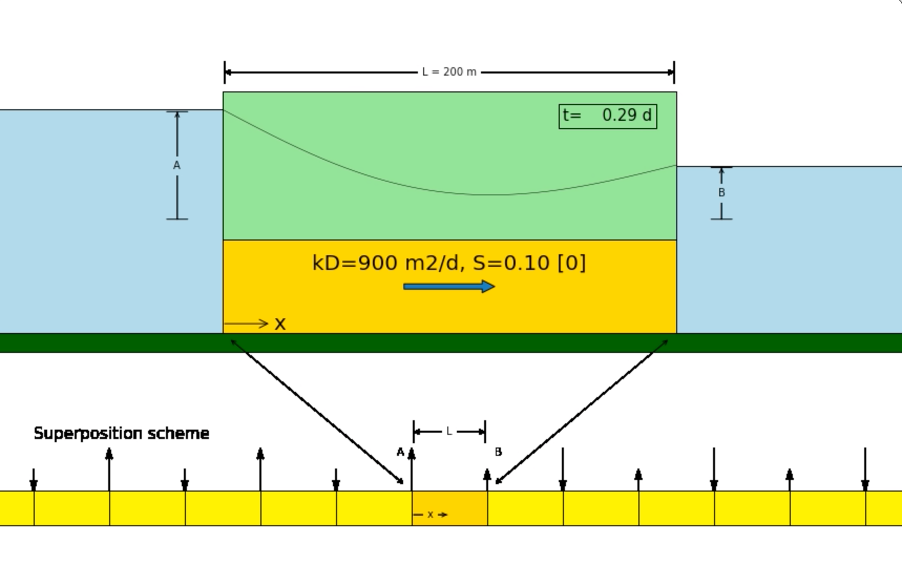
\includegraphics[width=0.8\textwidth]{pictures/2021_1}
\par\end{centering}
\caption{Strip of land bounded by fully penetrating surface water (top) and
superposition scheme (bottom).}
\end{figure}

\begin{enumerate}
\item Is this scheme correct? Explain why or why not that is the case. 
\end{enumerate}
\rule[0.5ex]{1\columnwidth}{1pt}

The scheme is correct because around the left ditch all mirror ditches
cancel out except so that at the left ditch, only het head change
at the left ditch remains. The same is true for the right ditch.

The first term of formula for drainage of a strip of land in which
the head is at $t=0$ is uniform and equal to $A$ m above the ditches
on either side is given by

\[
s\left(x,t\right)=A\frac{4}{\pi}\cos\left(\frac{\pi x}{2b}\right)\exp\left(-\left(\frac{\pi}{2}\right)^{2}\frac{t}{T}\right)\mbox{, with }T=\frac{b^{2}S}{kD}
\]

\rule[0.5ex]{1\columnwidth}{1pt}
\begin{enumerate}
\item What does this equation tell you? What's happening here? What name
would you give to \emph{T} ? Also explain why. 
\end{enumerate}
\rule[0.5ex]{1\columnwidth}{1pt}

The head between the diches has the shape of a cosine between $-\pi/2$
and $+\pi/2$ that declines exponentially with time. \emph{$T$} can
be named characteristic time because its scales the actual time.

\rule[0.5ex]{1\columnwidth}{1pt}
\begin{enumerate}
\item What is the halftime of this drainage process? Explain, and show it
mathematically. 
\end{enumerate}
\rule[0.5ex]{1\columnwidth}{1pt}

A halftime of a process is the time in which some outcome of the process
is halved. Halftimes are a characteristic of exponential decay.

Mathematically just say that $s_{t+\Delta t}=0.5s_{t}$, so

\[
\exp\left(-\left(\frac{\pi}{2}\right)^{2}\frac{t+\Delta t}{T}\right)=0.5\exp\left(-\left(\frac{\pi}{2}\right)^{2}\frac{t}{T}\right)
\]

\[
-\left(\frac{\pi}{2}\right)^{2}\frac{t+\Delta t}{T}=\ln2+0.5\left(\frac{\pi}{2}\right)^{2}\frac{t}{T}
\]

\[
\frac{\Delta t}{T}=\left(\frac{2}{\pi}\right)^{2}\ln2\approx0.28
\]

\rule[0.5ex]{1\columnwidth}{1pt}
\begin{enumerate}
\item How would you compare the rate of drainage of a desert that is 500
km wide between surface -water boundaries and an arable field of 100
m wide between ditches, if both have the same aquifer properties? 
\end{enumerate}
\rule[0.5ex]{1\columnwidth}{1pt}

The characteristic time is $T=\frac{b^{2}S}{kD}$, therefore,

\[
\frac{T_{\mathrm{desert}}}{T_{\mathrm{field}}}=\frac{b_{\mathrm{desert}}^{2}}{b_{\mathrm{field}}^{2}}=\frac{5^{2}\times10^{10}}{100^{2}}=25\times10^{6}
\]

\rule[0.5ex]{1\columnwidth}{1pt}

\subsection{Question 3}

The simplified Theis solution for the drawdown due to a pumping well
in a (un)confined aquifer reads

\[
s\left(r,t\right)=\frac{2.3Q}{4\pi kD}\log\left(\frac{2.25kDt}{r^{2}S}\right)
\]

A pumping test was carried out with an extraction of $Q=2400\,\mathrm{m^{3}/d}$.
The drawdown was measured in 3 observation wells.

The figure shows the measured drawdown $s$ in the observation wells
as a function of $t/r^{2}$ on logarithmic scale.

Answer the following questions
\begin{enumerate}
\item What is the transmissivity, explain and compute it. 
\end{enumerate}
\rule[0.5ex]{1\columnwidth}{1pt}

The drawdown per log-cycle is about 0.55 m, which should equal

\[
s_{10t}-s_{t}=\frac{2.3Q}{4\pi kD}\left[\log\left(\frac{2.25kD10t}{r^{2}S}\right)-\log\left(\frac{2.25kDt}{r^{2}S}\right)\right]
\]

\[
s_{10t}-s_{t}=\frac{2.3Q}{4\pi kD}\log\left(10\right)=\frac{2.3Q}{4\pi kD}=\frac{2.3\times2400}{4\pi kD}
\]

Therefore,

\[
kD\approx800\,\mathrm{m^{2}/d}
\]

\rule[0.5ex]{1\columnwidth}{1pt}
\begin{enumerate}
\item What is the storage coefficient, explain and compute it? 
\end{enumerate}
\rule[0.5ex]{1\columnwidth}{1pt}

Extending the straight portion of the drawdown curve to $s=0$ gives
$t/r^{2}=10^{-4}$. At this value, the argument of the logarithm must
be 1, because then the computed drawdown is zero.

\[
\frac{2.25kDt}{r^{2}S}=1=\frac{2.24kD}{S}\times10^{-4}
\]

\[
S=2.25\times800\times10^{-4}=0.018
\]

\rule[0.5ex]{1\columnwidth}{1pt}
\begin{enumerate}
\item If you had only the drawdown in the well itself instead of in observation
wells? What could you and what could you not determine, and why? 
\end{enumerate}
\rule[0.5ex]{1\columnwidth}{1pt}

In that case we can always compute the transmissivity, but not the
storage coefficient, because the drawdown in the well depends on other
things like borehole skin and partial penetration of the screen, which
are not known in general.

\rule[0.5ex]{1\columnwidth}{1pt}
\begin{enumerate}
\item What is the radius of influence? Explain and show it mathematically. 
\end{enumerate}
\rule[0.5ex]{1\columnwidth}{1pt}

That's the radius at which the drawdown in the simplified Theis formula
is zero, so that then the argument of the logarithm is zero. In fact,
this is what we used above to computed the storage coefficient, hence

\[
\frac{2.25kDt}{r^{2}S}=1\mbox{, so that }r=\sqrt{\frac{2.25kDt}{S}}
\]

\rule[0.5ex]{1\columnwidth}{1pt}

\section{Closed book reexam (1h), March 2018}

\subsection{Question 1:}
\begin{enumerate}
\item Explain what barometer efficiency (BE) is and how it physically works.
\item Explain in words what the characteristic halftime of an aquifer system
says about the behavior of the system?
\item Consider the parameters $L$ (system width), $kD$ (transmissivity)
and $S_{y}$ (specific yield), for each of these three parameters,
does in increase make the characteristic time larger or smaller?
\item What is capillary rise and what has capillary rise to do with air-entry
pressure?
\item When we extract water from a well in an infinitely extended aquifer,
from where does all this extracted water come? Explain your answer.
\end{enumerate}
\rule[0.5ex]{1\columnwidth}{1pt}
\begin{enumerate}
\item Barometer efficiency is the head decline due to barometer pressure
increase, both expressed in pressure of head\\
\[
BE=-\rho g\frac{\Delta\phi}{\Delta p}
\]
\item Characteristic half time of a groundwater system is the time during
which the head above the fixed boundary is halved due to natural drainage
alone. The characteristic time can be expressed as\\
\[
T=\frac{L^{2}S}{4kD}=\frac{b^{2}S}{kD}
\]
\item The L increases the halftime, like the S and the kD decreases the
halftime as follows from the formula.
\item Capillary rise is the suction of water from the saturated zone into
the unsaturated pore space. The air-entry pressure corresponds to
the larger pores and hence to the thickness of the capillary zone.
\item All the extracted water comes from storage.
\item This is due to the volume in the system relative to the drainage rate.
\end{enumerate}
\rule[0.5ex]{1\columnwidth}{1pt}

\subsection{Question 2:}

Consider an aquifer in direct contact with the ocean. The tide of
the ocean has an amplitude of $A=1.0\:\mathrm{m}$ and the cycle time
is $T=0.5\,\mathrm{d}$ (one full tide in 12h). The aquifer is confined.
The aquifer has the following properties: transmissivity $kD=900\,\mathrm{m^{2}/d}$
and storage coefficient $S_{y}=0.002$. We are only interested in
the effect of the tide land-inwards. The effect of the tidal fluctuation
on the groundwater head land-inward, $s$, obeys the following expression:

\[
s=A\,e^{-ax}\cos\left(\omega t-ax\right)\mbox{, where }a=\sqrt{\frac{\omega S}{2kD}}\mbox{, with }\omega=\frac{2\pi}{T}
\]

Notice that the difference between the uppercase \emph{S} and lowercase
\emph{s}.
\begin{enumerate}
\item Explain the parameters in the expression and given their dimension
\end{enumerate}
\rule[0.5ex]{1\columnwidth}{1pt}
\begin{description}
\item [{$s$:}] drawdown {[}L{]}
\item [{$A$:}] amplitude {[}L{]}
\item [{$x$:}] distance to where amplitude is given {[}L{]}
\item [{$a$:}] damping {[}L\textsuperscript{-1}{]}
\item [{$\omega$:}] angular velocity {[}radians/T{]} = {[}T\textsuperscript{-1}{]}
\item [{$T$:}] cycle time {[}T{]}
\end{description}
\rule[0.5ex]{1\columnwidth}{1pt}
\begin{enumerate}
\item What is the amplitude of the groundwater head fluctuation at 750 m
from the ocean? Explain your answer in a few words and fist show it
mathematically.
\end{enumerate}
\rule[0.5ex]{1\columnwidth}{1pt}

The amplitude only considers the damping, not the cosine,

\[
s=A\,e^{-ax}
\]

Just fil in the values.

\rule[0.5ex]{1\columnwidth}{1pt}
\begin{enumerate}
\item What is the delay of the head wave at 750 m from to the ocean with
respect to the tide? Hint: compute the velocity of the tidal wave
in the aquifer and then the time until the peak of the wave starting
at the ocean reaches $x=750\,\mathrm{m}$. Explain in a few words
your approach and start with showing your answer mathematically.
\end{enumerate}
\rule[0.5ex]{1\columnwidth}{1pt}

Delay requires knowledge of the wave velocity. The velocity is obtained
by realizing that the argument of the cosine must be constant when
following the wave at its own speed

\[
\omega t-ax=\mathrm{const}
\]

Take the derivative with respect to time

\[
\omega-a\frac{dx}{dt}=0
\]

or

\[
\frac{dx}{dt}=\frac{\omega}{a}
\]

The delay then is

\[
\Delta t=\frac{a}{\omega}\Delta x
\]

The delay at $x=L$ is obtained by setting $\Delta x=L$.

For the point at $L=750\,m$, we have

\[
\Delta t_{1}=\frac{a_{1}}{\omega}L_{1}
\]

Just fill in the numbers.

\rule[0.5ex]{1\columnwidth}{1pt}

\subsection{Question 3}

Consider a well in an infinite water-table (phreatic) aquifer. Drawdowns
are small compared to the thickness of the aquifer, so that $kD=900\,\mathrm{m^{2}/d}$
may be considered constant. The specific yield, $S_{y}=0.15$, is
also constant. As there are no boundary conditions, the drawdown by
the well follows the Theis equation. An approximation of which is

\[
s=\frac{Q}{4\pi kD}\ln\left(\frac{2.25kDt}{r^{2}S}\right)
\]

\begin{enumerate}
\item Derive a mathematical expression for the so-called \uline{radius
of influence}, that is, the distance beyond which the drawdown can
be neglected at a given time $t$. Notice that $\ln\left(\cdots\right)=2.3\log\left(\cdots\right)$.
\end{enumerate}
\rule[0.5ex]{1\columnwidth}{1pt}

The mathematical expression for the radius of influence is obtained
by computing the radius for which the drawdown computed by this simplified
formula is zero. That is for which the argument of the logarithm is
1.

\[
\frac{2.25kDt}{r^{2}S}=1
\]

so that

\[
r=\sqrt{\frac{2.25kDt}{S}}
\]

\rule[0.5ex]{1\columnwidth}{1pt}
\begin{enumerate}
\item As you can see from the equation, the drawdown is (approximately)
a logarithmic function in time. Derive a mathematical expression of
the increase of the drawdown per log cycle of time, that is, between
time \emph{t} and time 10\emph{t.}.
\end{enumerate}
\rule[0.5ex]{1\columnwidth}{1pt}

Simply subtract the drawdown at time $10t$ from that at time $t$

\[
s_{10t}-s_{t}=\frac{2.3Q}{4\pi kD}\left[\log\left(\frac{2.25kD10t}{r^{2}S}\right)-\log\left(\frac{2.25kDt}{r^{2}S}\right)\right]=\frac{2.3Q}{4\pi kD}
\]

\rule[0.5ex]{1\columnwidth}{1pt}
\begin{enumerate}
\item The figure below shows an example of an actual drawdown measured at
a piezometer at \emph{r} = 100 m from the well extracting $Q=1200\,\mathrm{m^{3}/d}$.
Determine the transmissivity of the aquifer.
\end{enumerate}
\begin{figure}
\begin{centering}
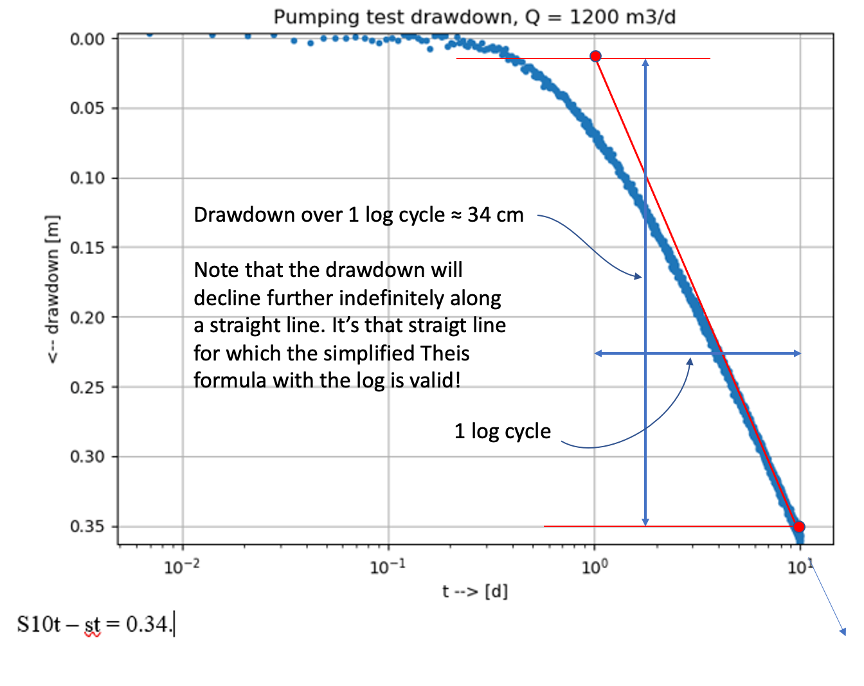
\includegraphics[width=0.8\textwidth]{pictures/2018_2}
\par\end{centering}
\caption{Measured drawdown in piezometer at \emph{$r=100\,\mathrm{m}$} from
well extracting $Q=1200\,\mathrm{m^{3}/d}$}
\end{figure}

\rule[0.5ex]{1\columnwidth}{1pt}

The drawdown per log cycle is 0.34 m. Hence,

\[
s_{10t}-s_{t}=0.34=\frac{2.3Q}{4\pi kD}
\]

and so,

\[
kD=\frac{2.3Q}{4\pi\left(s_{10t}-s_{t}\right)}=\frac{2.3\times1200}{4\pi0.34}\approx645\,\mathrm{m^{2}/d}
\]

\rule[0.5ex]{1\columnwidth}{1pt}
\begin{enumerate}
\item Bonus question (extra points): Determine the storage coefficient.
\end{enumerate}
\rule[0.5ex]{1\columnwidth}{1pt}

The storage coefficient is obtained from the intersection of the tangent
to the straight part of the graph with s=0, hence for which the argument
of the log is 1.

\[
\frac{2.25kDt}{r^{2}S}=1
\]

Therefore, with intersection time at $t_{0}\approx1.0\,\mathrm{d}$

\[
S=\frac{2.25kDt_{0}}{r^{2}}=\frac{2.25\times625\times1.0}{100^{2}}=0.14
\]

\rule[0.5ex]{1\columnwidth}{1pt}

\section{Closed book exam (1h), Feb 7, 2017}

\subsection{Question 1:}
\begin{enumerate}
\item Someone says the barometer efficiency of the piezometer in his garden
is 25\%. What does that mean? Explain your answer telling how this
phenomenon physically works. 
\end{enumerate}
\rule[0.5ex]{1\columnwidth}{1pt}

A barometer efficiency of 25\% implies a loading efficiency of 75\%,
i.e., that 75\% of the load increment on ground surface is carried
by the water and the remaining 25\% by the soil skeleton. The increase
of the pressure by 75\% due to a load means a water table rise of
75\% in the piezometer, however because it is the barometer that causes
the load increase, the full 100\% of the barometer pressure increase
works on the water surface in the piezometer, so that the net effect
for the water level is 75\% up + 100\% down = 25\% down in the piezometer.

\rule[0.5ex]{1\columnwidth}{1pt}
\begin{enumerate}
\item A pressure logger that is installed in this piezometer measures absolute
pressure. What is absolute pressure? And what does this pressure gauge
see when the barometer rises by the equivalent of 40 cm of water column,
given the barometric efficiency of 25\%? 
\end{enumerate}
\rule[0.5ex]{1\columnwidth}{1pt}

The loading efficiency $LE=1-BE=75%\ensuremath{\%}
$. This is what is registered by the piezometer, $0.75\times40\,\mathrm{cm}=30\,\mathrm{cm}$
equivalent pressure rise.

\rule[0.5ex]{1\columnwidth}{1pt}
\begin{enumerate}
\item What properties determine the value of the specific (elastic) storage
coefficient? 
\end{enumerate}
\rule[0.5ex]{1\columnwidth}{1pt}

The loading efficiency, i.e., the compressibility of the water and
that of the skeleton of the aquifer matrix material.

\rule[0.5ex]{1\columnwidth}{1pt}
\begin{enumerate}
\item What does the air-entry value have to do with the thickness of the
capillary fringe/zone? Explain your answer. 
\end{enumerate}
\rule[0.5ex]{1\columnwidth}{1pt}

The air-entry pressure corresponds to the thickness of the full capillary
zone as it is the pressure required to blow air through the largest
pores. So, this pressure corresponds to the capillary rise that matches
the diameter of these largest pores.

The transient drawdown of a well with a constant extraction \emph{Q}
in the case without any head boundary condition is mathematically
described by the Theis well drawdown:

\[
s=\frac{Q}{4\pi kD}\mathrm{W}\left(\frac{r^{2}S}{4kDt}\right)
\]

that can be approximated by

\[
s\approx\frac{Q}{4\pi kD}\ln\left(\frac{2.25kDt}{r^{2}S}\right)
\]

\rule[0.5ex]{1\columnwidth}{1pt}
\begin{enumerate}
\item Sketch both graphs such that s is on a linear scale (downward positive)
and time on a logarithmic horizontal scale. What's the difference
between the two? 
\end{enumerate}
\rule[0.5ex]{1\columnwidth}{1pt}

A straight line (approximation) and a straight line that deviates
asymptotically to zero for small drawdowns (Theis).

\rule[0.5ex]{1\columnwidth}{1pt}
\begin{enumerate}
\item What is the drawdown per log-cycle of time, assuming that the approximation
is valid? 
\end{enumerate}
\rule[0.5ex]{1\columnwidth}{1pt}

Just ask what is $s_{10t}-s_{t}$:

\[
s_{10t}-s_{t}=\frac{Q}{4\pi kD}\ln10=\frac{2.3Q}{4\pi kD}\log10=\frac{2.3Q}{4\pi kD}
\]

\rule[0.5ex]{1\columnwidth}{1pt}
\begin{enumerate}
\item What does `adius of influence` mean; how could you derive it from
the above approximation? 
\end{enumerate}
\rule[0.5ex]{1\columnwidth}{1pt}

The distance where $s(r,t)=0$, i.e., set the argument of the log
to one:

\[
s=0\rightarrow\frac{2.25kDt}{r^{2}S}=1\rightarrow r=\sqrt{\frac{2.25kDt}{S}}
\]

\rule[0.5ex]{1\columnwidth}{1pt}
\begin{enumerate}
\item Does the Theis drawdown reach a steady-state situation in the long
run? Explain your answer. 
\end{enumerate}
\rule[0.5ex]{1\columnwidth}{1pt}

The Theis drawdown has not steady state solution because all the pumped
water comes from storage

\rule[0.5ex]{1\columnwidth}{1pt}

We know the total discharge (flow) across a ring at fixed distance
\emph{r} from the well in a confined aquifer is given by

\[
Q_{r,t}=Q_{0}\,e^{-u}\mbox{, with }u=\frac{r^{2}S}{4kDt}
\]

\begin{enumerate}
\item If you assume you are at a fixed distance r from the well, could you
then formulate a characteristic time for the transient phenomenon
$Q(r,t)$? Explain your answer. 
\end{enumerate}
\rule[0.5ex]{1\columnwidth}{1pt}

Just set 
\[
u=\frac{r^{2}S}{4kDt}=\frac{T}{t}\rightarrow T=\frac{r^{2}S}{4kDt}
\]

\rule[0.5ex]{1\columnwidth}{1pt}

Below, we observe a hydrologist interpreting a transient pumping test
in a confined aquifer. He/she plotted the drawdown data on a double
log graph with drawdown \emph{s} vertically upward and $t/r^{2}$
horizontally. The data of this graph with the measurements was then
shifted over the Theis type-curve until the best possible match was
obtained. This match is shown in the figure. Given that the extraction
during the pumping test was $Q=1200\,\mathrm{m^{3}/d}$.
\begin{enumerate}
\item Determine the transmissivity $kD$ and the storage coefficient $S$.
\end{enumerate}
\begin{figure}
\begin{centering}
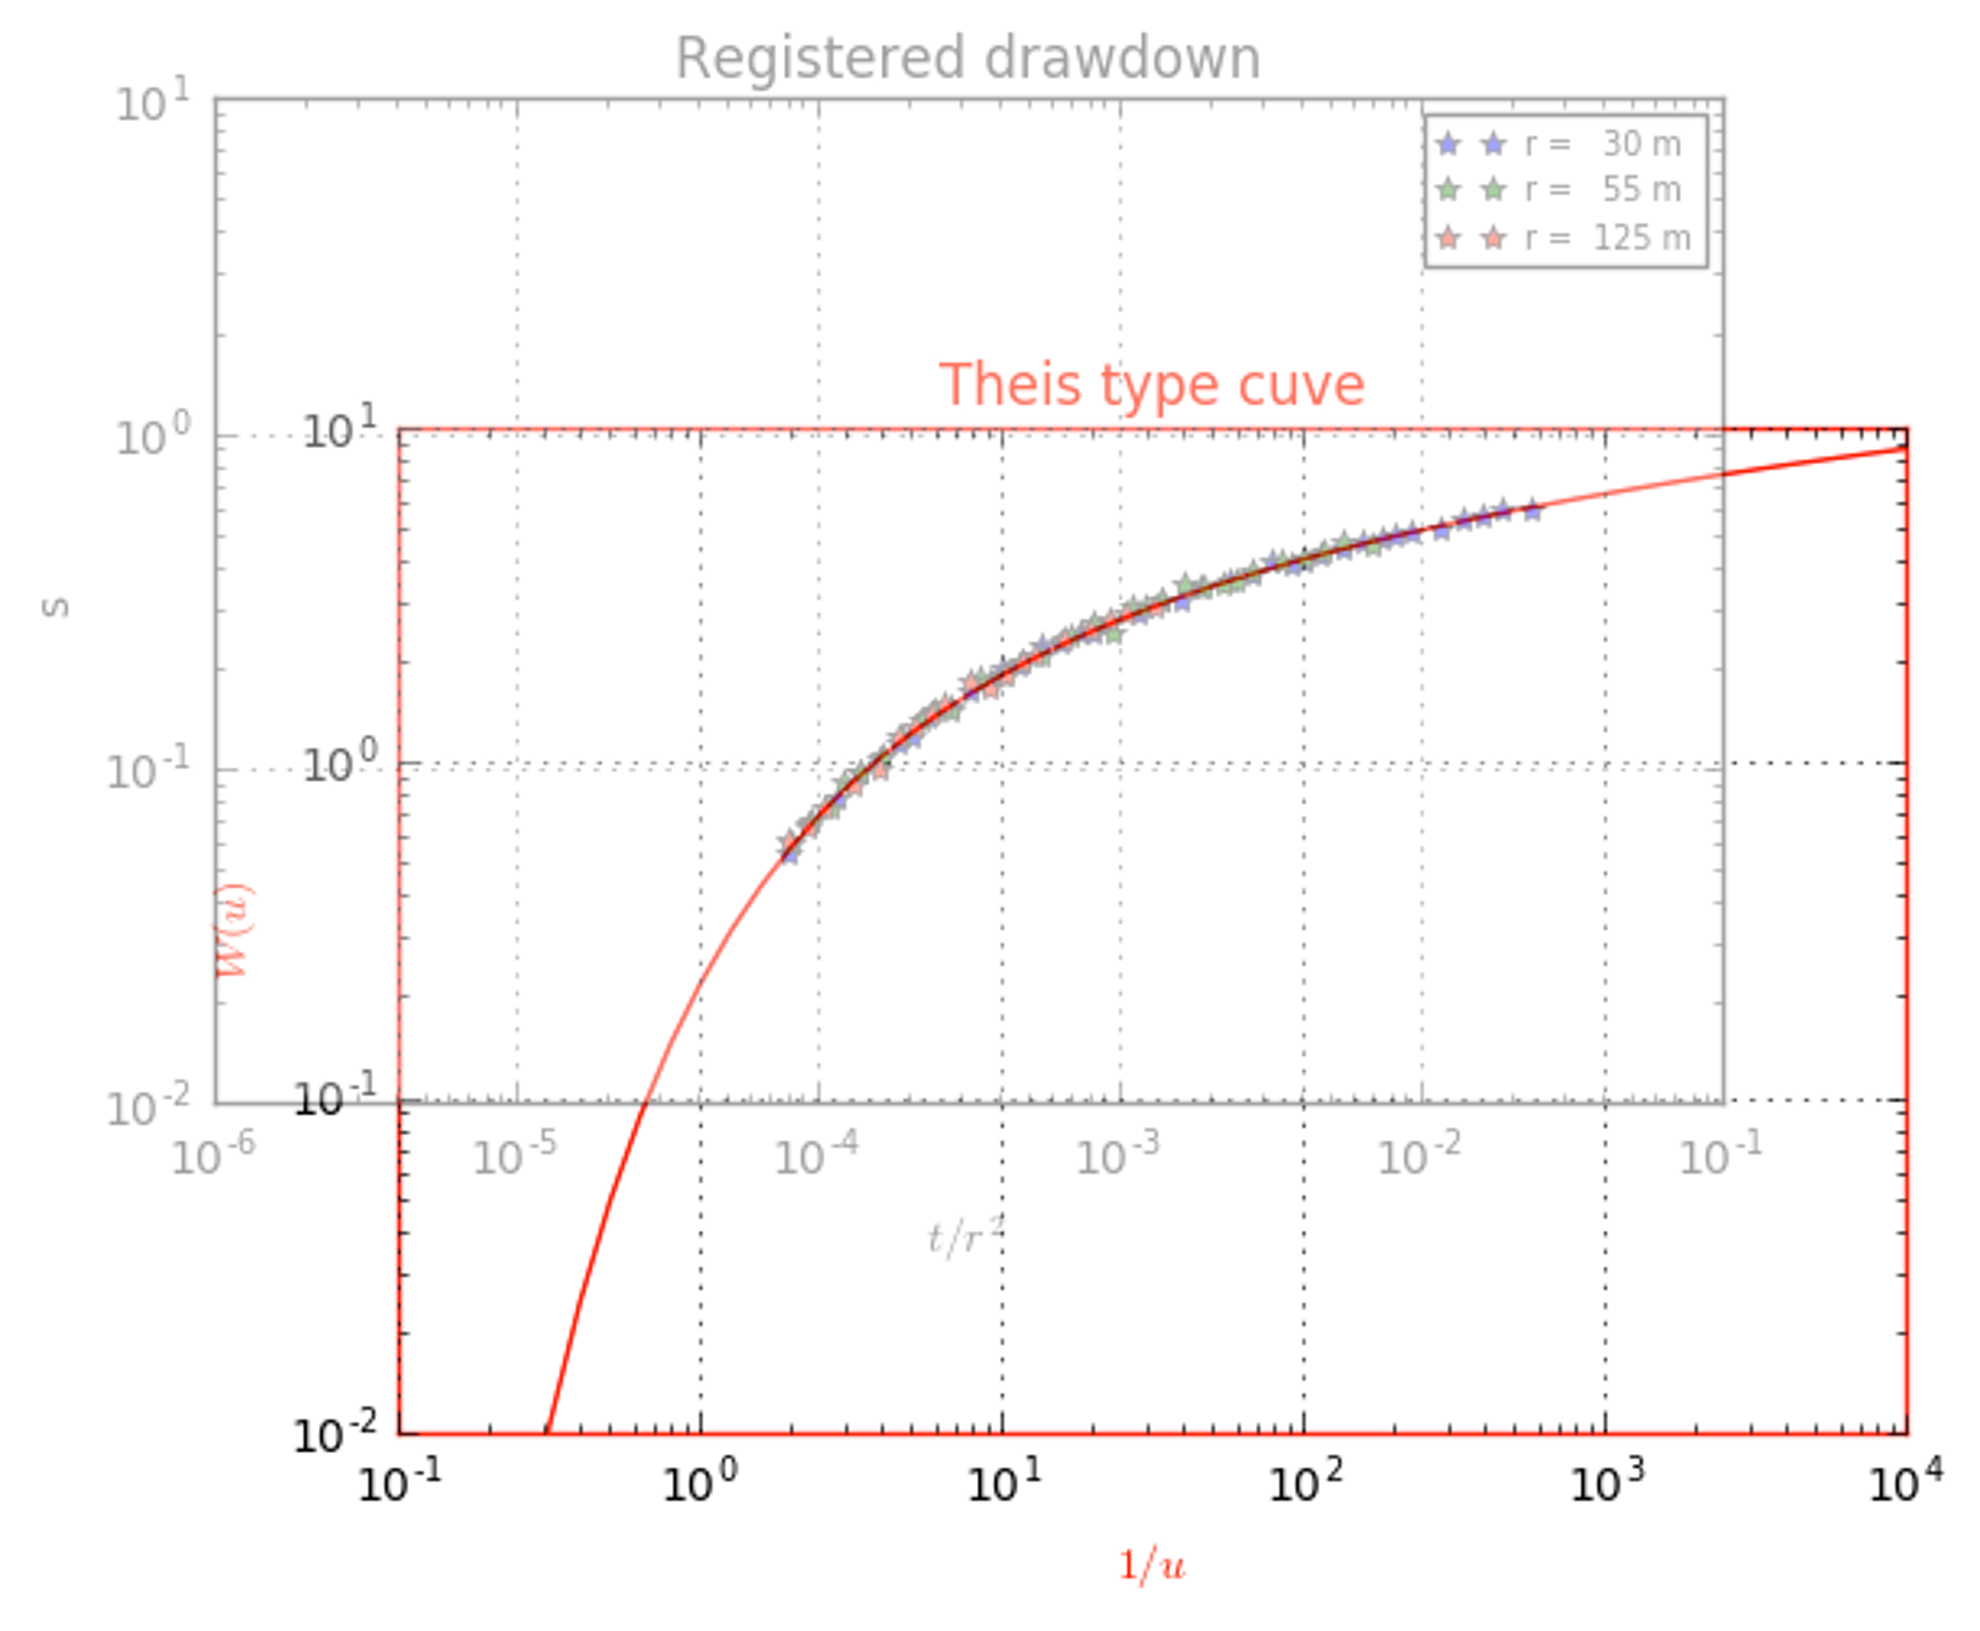
\includegraphics[width=1\textwidth]{pictures/2017_1}
\par\end{centering}
\caption{Measured drawdown curve matched with Theis type curve.}
\end{figure}

\rule[0.5ex]{1\columnwidth}{1pt}

Take two corresponding points on the vertical axis e.g.

\[
s=0.1\mbox{and }\mathrm{W}\left(u\right)=0.9
\]

And on the horizontal axis:

\[
\frac{1}{u}=0.1\mbox{ and }\frac{t}{r^{2}}=4\times10^{-6}
\]

Then

\[
\frac{s}{\mathrm{W\left(u\right)}}=\frac{Q}{4\pi kD}\rightarrow\frac{0.1}{0.9}=\frac{1200}{4\pi kD}\rightarrow kD=860\,\mathrm{m^{2}/d}
\]

and

\[
\frac{1}{u}=\frac{4kD}{S}\frac{t}{r^{2}}\rightarrow S=4kD\frac{t/r^{2}}{1/u}=4kD\frac{4\times10^{-6}}{0.1}=4\times860\times4\times10^{-5}=0.14
\]

\rule[0.5ex]{1\columnwidth}{1pt}

\subsection{Question 3:}

Imagine the sea tide acting on a shore that has a confined aquifer
inland with a constant \emph{$kD$} and \emph{$S$} in good vertical
contact with the sea. The tide waves, which are characterized by \emph{$A$}
and $\omega$, therefore, penetrate the aquifer; they are mathematically
described by:

\[
s_{x,t}=A\,e^{-ax}\sin\left(\omega t-ax\right)
\]

\begin{enumerate}
\item As can be seen, this equation describes two simultaneous phenomena.
Which are these two phenomena? 
\end{enumerate}
The factor \emph{$a$} in the equation was derived to be

\[
a=\sqrt{\frac{\omega S}{2kD}}
\]

Damping of the wave with x and 
\begin{enumerate}
\item What are the parameters with their dimensions? 
\end{enumerate}
\rule[0.5ex]{1\columnwidth}{1pt}
\begin{description}
\item [{$s$:}] is the change of head relative to mean due to wave {[}m{]}
\item [{$A$:}] is wave amplitude {[}m{]}
\item [{$\omega$:}] is frequency, {[}rad/day{]} or {[}1/day{]}
\item [{$S$:}] is storage coeffiicient {[}-{]}
\item [{$kD$:}] is transmissivity {[}m$^{2}$/d{]}
\item [{$a$:}] damping {[}1/m{]}
\end{description}
\rule[0.5ex]{1\columnwidth}{1pt}
\begin{enumerate}
\item A tidal wave has a frequency $\omega$ of two cycles per day of 24
hours, or a cycle time $T$ of 12 hours. Large wind waves, however,
have a cycle time of only about 12 seconds. How far does the influence
of these wind waves penetrate into the aquifer compared to the influence
of the tide waves? Give their ratio and sketch the envelope of both
to show this difference (the sketch does not have to be on scale). 
\end{enumerate}
\rule[0.5ex]{1\columnwidth}{1pt}

The ratio of the damping due to different frequencies is, with index
1 referring to the low tidal frequency and index 2 to the fast wave
frequency:

\[
\frac{a_{1}}{a_{2}}=\sqrt{\frac{\omega_{1}}{\omega_{2}}}=\sqrt{\frac{T_{2}}{T_{1}}}=\sqrt{\frac{12\,\mathrm{s}}{12\times3600\,\mathrm{s}}}=\sqrt{\frac{1}{3600}}=\frac{1}{60}
\]

So that the damping of the fast wind wave is 60 times more that that
of the slow tidal wave.

\rule[0.5ex]{1\columnwidth}{1pt}

\section{Closed book reexam (1h), Feb 2016}

\subsection{Question 1:}
\begin{enumerate}
\item Explain what barometer efficiency ($BE$) is and how it physically
works. 
\item Explain in words what the characteristic (half) time of a groundwater
system is. What does is say about the behavior of the system?
\item For which of the parameters $L$ (system width), $kD$ (transmissivity)
and $S_{y}$ (specific yield) would an increase make the characteristic
system time smaller?
\item Explain why in hydrological logic you think that this is the case. 
\item If you see a close-up of two grains held together by a small amount
of water at their point of contact. What then is the pressure in that
water? Explain why that is so. 
\end{enumerate}
\rule[0.5ex]{1\columnwidth}{1pt}
\begin{enumerate}
\item Barometer efficiency is the head decline due to barometer pressure
increase, both expressed in pressure of head\\
\[
BE=-\rho g\frac{\Delta\phi}{\Delta p_{a}}
\]
\item Characteristic half time of a groundwater system is the time during
which the head above the fixed boundary is halved due to natural drainage
alone. The characteristic time can be expressed as\\
\[
T=\frac{L^{2}S}{kD}
\]
\item Hence it is 4 times as long for a system with a double width; it is
proportional to the storage coefficient and inversely proportional
to the transmissivity of the groundwater system.
\item This is due to the volume in the system relative to the drainage rate.
\item The curvature of the free water surface between the grains shows that
the pressure must be negative, which causes the cohesion between the
grains.
\end{enumerate}
\rule[0.5ex]{1\columnwidth}{1pt}

\subsection{Question 2:}

Consider an aquifer in direct contact with the ocean. The tide of
the ocean has an amplitude $A=1.0\,\mathrm{m}$ and the cycle time
is $T=0.5\,\mathrm{d}$ (one full tide in 12h). The aquifer is confined.
It consists of two parts. The first part reaches from the ocean to
500 m inland, the second part is present at more than 500 m from the
ocean. The first part of the aquifer has the following properties:
transmissivity $kD=900\,\mathrm{m^{2}/d}$ and storage coefficient
$S=0.002$. The second part of the aquifer has the following properties:
$kD=1800\,\mathrm{m^{2}/d}$ and storage coefficient $S=0.001$. Because
we consider the fluctuation of the head to be superposed on the mean
head, we are only interested in the head $s$ relative to the mean
head at every location, that is, in $s\left(x,t\right)=h\left(x,t\right)-h\left(x\right)$.
This head fluctuation, $s,$ obeys following expression:

\[
s=A\,e^{-ax}\cos\left(\omega t-ax\right)\mbox{, where }a=\sqrt{\frac{\omega S}{2kD}}\mbox{ and }\omega=\frac{2\pi}{T}
\]

Notice that the storage coefficient is capital $S$ and the head relative
to the mean head is lowercase $s$.
\begin{enumerate}
\item Explain the parameters in the expression and given their dimension
\end{enumerate}
\rule[0.5ex]{1\columnwidth}{1pt}
\begin{description}
\item [{$s$:}] drawdown {[}L{]}
\item [{$A$:}] amplitude {[}L{]}
\item [{$x$:}] distance to where amplitude is given {[}L{]}
\item [{$a$:}] damping {[}L\textsuperscript{-1}{]}
\item [{$\omega$:}] angular velocity {[}radians/T{]} = {[}T\textsuperscript{-1}{]}
\item [{$T$:}] cycle time {[}T{]}
\end{description}
\rule[0.5ex]{1\columnwidth}{1pt}
\begin{enumerate}
\item What is the amplitude of the groundwater head fluctuation, that is,
the amplitude of $s$ in the aquifer at 500 m and at 1000 m from the
ocean? 
\end{enumerate}
\rule[0.5ex]{1\columnwidth}{1pt}

The amplitude only considers the damping, not the cosine,

\[
s=A\,e^{-ax}
\]

For the first part use aquifer properties of that part, yielding $s_{1}$
and fill in $x=L_{1}$ 

Hence,

\[
s_{1}=A\,e^{-aL_{1}}
\]

The amplitude at $x=L_{2}$ can be computed relative to that at $x=L_{1}$

\[
s_{2}=\left(A\,e^{-a_{1}L_{1}}\right)e^{-a_{2}\left(L_{2}-L_{1}\right)}
\]

\[
s_{2}=A\,e^{-a_{1}L_{1}-a_{2}\left(L_{2}-L_{1}\right)}
\]

\rule[0.5ex]{1\columnwidth}{1pt}
\begin{enumerate}
\item What is the delay of the head wave at 500 m and 1000 m relative to
the ocean tide? Hint: compute the velocity of the tidal wave in the
aquifer and then the time until the peak of the wave starting at the
ocean reaches $x=500\,\mathrm{m}$ and $x=1000\,\mathrm{m}$.
\end{enumerate}
\rule[0.5ex]{1\columnwidth}{1pt}

Delay requires knowledge of the wave velocity. The velocity is obtained
by realizing that the argument of the cosine must be constant when
following the wave at its own speed

\[
\omega t-ax=\mathrm{const}
\]

take the derivative with respect to time

\[
\omega-a\frac{dx}{dt}=0
\]

or

\[
\frac{dx}{dt}=\frac{\omega}{a}
\]

The delay then is

\[
\Delta t=\frac{a}{\omega}\Delta x
\]

The delay at $x=L_{1}$ is obtained by setting $\Delta x=L_{1}$

\[
\Delta t_{1}=\frac{a_{1}}{\omega}L_{1}
\]

For the point at $x=L_{2}$ we have

\[
\Delta t_{2}=\frac{a_{2}}{\omega}\left(L_{2}\right)
\]

Hence, the total delay up to the point $x=L_{1}+L_{2}$ would be

\[
\Delta t=\frac{a_{1}}{\omega}L_{1}+\frac{a_{2}}{\omega}L_{2}
\]

\rule[0.5ex]{1\columnwidth}{1pt}

\subsection{Question 3:}

Consider a well in an infinite water table (phreatic) aquifer. Drawdowns
are considered small compared to the thickness of the aquifer, so
that $kD=900\,\mathrm{m^{2}d}$ may be considered constant. The specific
yield, $S_{y}=0.15$, is also constant. As there are no boundary conditions,
the drawdown by the well follows the Theis equation. An approximation
of which is

\[
s\approx\frac{Q}{4\pi kD}\frac{2.3Q}{4\pi kD}\log\left(\frac{2.25kDt}{r^{2}S}\right)
\]

\begin{enumerate}
\item Derive a mathematical expression for the so-called radius of influence,
that is, the distance beyond which the drawdown can be neglected at
a given time $t$ after the well was first switched on.
\end{enumerate}
\rule[0.5ex]{1\columnwidth}{1pt}

The mathematical expression for the radius of influence is obtained
by computing the radius for which the drawdown computed by this simplified
formula is zero. That is for which the argument of the logarithm is
1.

\[
\frac{2.25kDt}{r^{2}S}=1
\]

so that

\[
r=\sqrt{\frac{2.25kDt}{S}}
\]

\rule[0.5ex]{1\columnwidth}{1pt}
\begin{enumerate}
\item As you can see, the drawdown is a logarithmic function in time. Derive
a mathematical expression of the increase of the drawdown per log
cycle, that is, between for instance $t=6\,\mathrm{d}$ and $t=60\,\mathrm{d}$,
or $t=2\,\mathrm{d}$ and $t=20\,\mathrm{d}$.
\end{enumerate}
\rule[0.5ex]{1\columnwidth}{1pt}

Simply subtract the drawdown at $t$ from that at $10t$

\[
s_{10t}-s_{t}=\frac{2.3Q}{4\pi kD}\left[\log\left(\frac{2.25kD\left(10t\right)}{r^{2}S}\right)-\log\left(\frac{2.25kDt}{r^{2}S}\right)\right]=\frac{2.3Q}{4\pi kD}
\]

\rule[0.5ex]{1\columnwidth}{1pt}
\begin{enumerate}
\item Assume the well has been continuously pumping for time $t=t$, after
which the extraction was stopped. What is the drawdown at distance
$r_{0}$ at time is $t=t_{1}+\Delta t$ , where $\Delta t$ is any
time passed since $t_{1}$.
\end{enumerate}
\rule[0.5ex]{1\columnwidth}{1pt}

The drawdown at $t+\Delta t$ is obtained by superposition of an extraction
\emph{$Q$} for the entire period from $t$ to $t+\Delta t$ and an
extraction of $-Q$ for the period between $t_{1}$ and $t_{1}+\Delta t$.
Hence,

\[
s=\frac{2.3Q}{4\pi kD}\left[\log\left(\frac{2.25kD\left(t_{1}+\Delta t\right)}{r_{0}^{2}S}\right)-\log\left(\frac{2.25kD\Delta t}{r_{0}^{2}S}\right)\right]
\]

\[
s=\frac{2.3Q}{4\pi kD}\log\left(\frac{t_{1}+\Delta t}{\Delta t}\right)
\]

Under the condition that the logarithmic expression is valid for the
considered point $r_{0}$ and times $t\ge t_{1}$, otherwise we must
apply the regular Theis equation, in which case we cannot simply combine
two logarithms.

\rule[0.5ex]{1\columnwidth}{1pt}

\section{Closed-book exam (1h), Feb 1, 2016}

\subsection{Question 1: (16 points)}
\begin{enumerate}
\item Explain loading efficiency, $LE$.
\end{enumerate}
\rule[0.5ex]{1\columnwidth}{1pt}

$LE$ is the ratio of the pressure increase of the water in the (confined)
aquifer and the pressure of the load on ground surface.

\rule[0.5ex]{1\columnwidth}{1pt}
\begin{enumerate}
\item Explain the barometer efficiency, $BE$.
\end{enumerate}
\rule[0.5ex]{1\columnwidth}{1pt}

The $BE$ is the ratio of the head decline measurable in a piezometer
in the confined aquifer over the pressure increase of the barometer,
both expressed in pressure units {[}N/m$^{2}${]}.

\rule[0.5ex]{1\columnwidth}{1pt}
\begin{enumerate}
\item What is the difference registered by a pressure gauge in a confined
aquifer measuring absolute pressure, given on the one hand a uniform
mass placed at ground surface of weight $\Delta p$ N/m\textsuperscript{2}
and on the other hand a barometer increase of the same value of $\Delta p\,\mathrm{N/m^{2}}$? 
\end{enumerate}
\rule[0.5ex]{1\columnwidth}{1pt}

The absolute pressure in the confined aquifer increases by the same
amount in both cases, i.e., $LE\times\Delta p$. Of course, the head
in the piezometer declines due to an increase of the barometer, but
not the absolute pressure in the aquifer. (Only one student had this
right).

\rule[0.5ex]{1\columnwidth}{1pt}
\begin{enumerate}
\item What is the origin of delayed yield? 
\end{enumerate}
\rule[0.5ex]{1\columnwidth}{1pt}

Delayed yield stems from delayed drawdown due to unconfined storage
that manifests itself after the drawdown due to elastic, which is
must faster due to the elastic storage coefficient that is about two
orders of magnitude smaller than the phreatic storage or specific
yield. Delayed yield may be encountered both in a phreatic aquifer
and in semi-confined aquifers with an overlaying phreatic water table
than cannot be maintained when it is affected by downward leakage
into the pumped semi-confined aquifer below.

\rule[0.5ex]{1\columnwidth}{1pt}
\begin{enumerate}
\item In which case does the influence of tide reach further inland into
an aquifer?
\end{enumerate}
The case with the higher or with the lower frequency? 

\rule[0.5ex]{1\columnwidth}{1pt}

The lower the frequency the further the reach, with zero frequency
(that is, steady state), the reach is theoretically infinite. In reverse,
with infinite frequency, the reach is zero, obviously.

\rule[0.5ex]{1\columnwidth}{1pt}

The case with the larger or the smaller transmissivity \emph{kD}? 

\rule[0.5ex]{1\columnwidth}{1pt}

The larger the \emph{kD} the farther the inland reach of the tide.
With infinite \emph{kD}, the reach is infinite, with zero \emph{kD}
the reach is zero, obviously.

\rule[0.5ex]{1\columnwidth}{1pt}

The case with the larger or with the smaller storage coefficient \emph{S}? 

\rule[0.5ex]{1\columnwidth}{1pt}

The smaller the storage coefficient, the farther the tidal fluctuation
reaches inland. With zero storage coefficient the reach is infinite,
and with infinite storage coefficient, the reach is zero, obviously.

\rule[0.5ex]{1\columnwidth}{1pt}
\begin{enumerate}
\item What is the difference between the situations with the wells that
were studied by Theis and by Hantush? 
\end{enumerate}
\rule[0.5ex]{1\columnwidth}{1pt}

Theis studies confined aquifers, including unconfined ones with constant
transmissivity, in general, aquifers without external sources, in
which all extracted water stems from storage alone.

Hantush studied semi-confined aquifers, aquifers in which the extracted
water stems both from storage and from leakage from an overlying layer
with constant head.

\rule[0.5ex]{1\columnwidth}{1pt}
\begin{enumerate}
\item Does the Theis case have a final equilibrium drawdown? Explain your
answer. 
\end{enumerate}
\rule[0.5ex]{1\columnwidth}{1pt}

Because all water in the Theis case comes from storage there is no
steady-stage drawdown possible.

\rule[0.5ex]{1\columnwidth}{1pt}
\begin{enumerate}
\item Does the Hantush case have a final, steady-state drawdown? Explain
your answer. 
\end{enumerate}
\rule[0.5ex]{1\columnwidth}{1pt}

Because the part of the water from the overlaying layer is proportional
to drawdown, there will be equilibrium in the end. So yes, there exists
a st

\rule[0.5ex]{1\columnwidth}{1pt}

\subsection{Question 2: (14 points)}
\begin{enumerate}
\item Explain what is the radius of influence of an extraction well in an
aquifer of constant transmissivity and storage coefficient? 
\end{enumerate}
\rule[0.5ex]{1\columnwidth}{1pt}

The radius of influence is the radius beyond which the (transient)
drawdown is negligible. 

\rule[0.5ex]{1\columnwidth}{1pt}
\begin{enumerate}
\item The simplified Theis solution is as follows:\\
\[
s\left(r,t\right)\approx\frac{Q}{4\pi kD}\ln\left(\frac{2.25kDt}{r^{2}S}\right)
\]
From it derive an expression of the radius of influence.
\end{enumerate}
\rule[0.5ex]{1\columnwidth}{1pt}

Set the argument of the log to 1 so that the log and with it the drawdown
becomes zero. Then\\
\[
\frac{2.25kDt}{r^{2}S}=1\rightarrow r=\sqrt{\frac{2.25kDt}{S}}
\]

\rule[0.5ex]{1\columnwidth}{1pt}
\begin{enumerate}
\item Also show what is the drawdown difference per log cycle of time, that
is, between time is $t$ and time is $10t$. 
\end{enumerate}
\rule[0.5ex]{1\columnwidth}{1pt}

The drawdown difference per log cycle (not ratio as some of you assumed)
is

\[
s_{10t}-s_{t}=\frac{Q}{4\pi kD}\left[\ln\left(\frac{2.35kD\left(10t\right)}{r^{2}S}\right)-\ln\left(\frac{2.25kDt}{r^{2}S}\right)\right]=\frac{Q}{4\pi kD}\ln10=\frac{2.3Q}{4\pi kD}
\]

\rule[0.5ex]{1\columnwidth}{1pt}
\begin{enumerate}
\item Consider a well in a water table aquifer at 300 m from an impervious
wall that reaches to the bottom of the aquifer. The aquifer has $kD=600\,\mathrm{m^{2}d}$
and the specific yield of $S_{y}=0.2$. The pumping rate is $Q=1200\,\mathrm{m^{3}/d}$.
Assume that the approximation of the Theis equation that is given
in this question is applicable. Compute the head change of the groundwater
at the wall closest to the well. 
\end{enumerate}
\rule[0.5ex]{1\columnwidth}{1pt}

Due to the presence of an impervious wall, we must use a mirror well
that guarantees that there is no flow perpendicular to the wall. This
mirror well must be placed on the other side of the wall at the same
distance and its flow must be equal in both quantity and sign as that
of the real well. The resulting drawdown is then the superposition
of that of the well and its mirror well.

\[
s=\frac{Q}{4\pi kD}\ln\left(\frac{2.25kDt}{r_{1}^{2}S}\right)+\frac{Q}{4\pi kD}\ln\left(\frac{2.25kDt}{r_{2}^{2}S}\right)
\]

\[
s=\frac{Q}{4\pi kD}\ln\left(\left[\frac{2.25kDt}{r_{1}r_{2}S}\right]^{2}\right)
\]

\[
s=\frac{Q}{2\pi kD}\ln\left(\frac{2.25kDt}{r_{1}r_{2}S}\right)
\]

with $r=r_{1}=r_{2}=300\,\mathrm{m}$, so that

\[
s=\frac{Q}{2\pi kD}\ln\left(\frac{2.25kDt}{r^{2}S}\right)
\]

Just fill in the provided numbers to get the numerical answer.

\rule[0.5ex]{1\columnwidth}{1pt}

\section{Close-book exam (1h), Feb 2015}

\subsection{Question 1:}
\begin{enumerate}
\item What types of storage or storage coefficients are associated with
transient groundwater flow? And explain short how they physically
work. 
\end{enumerate}
\rule[0.5ex]{1\columnwidth}{1pt}
\begin{enumerate}
\item Elastic storage, from expansion and shrinking of the volume of the
water ands the porous medium under changes of water and grain pressure. 
\item Storage from decline of the water table, i.e., drainage of pores,
drainage from the unsaturated zone.
\end{enumerate}
\rule[0.5ex]{1\columnwidth}{1pt}
\begin{enumerate}
\item Explain the relation between capillary rise and pore diameter.
\end{enumerate}
\rule[0.5ex]{1\columnwidth}{1pt}

Capillary rise is the net effect of attraction between water and grain
surface (cohesion) and gravity. It may be expressed as upward attraction
equals downward gravity force:

\[
2\pi r\sigma\cos\gamma=\pi r^{2}\rho gh
\]

Hence the capillary rise is inversely proportional to the effective
pore radius \emph{r}

\[
h=\frac{2\pi\sigma\cos\gamma}{\pi r^{2}\rho g}=\frac{1}{r}\frac{2\sigma\cos\gamma}{\rho g}
\]

\rule[0.5ex]{1\columnwidth}{1pt}
\begin{enumerate}
\item Explain the general shape of the moisture curve in the unsaturated
zone. Describe where the water comes from when the water table is
lowered. 
\end{enumerate}
\rule[0.5ex]{1\columnwidth}{1pt}

The general shape of the moisture curve is straight at porosity upward
from the water table to the top of the capillary zone and then declining
upward as more and more pores fall dry depending on their pore size.
At each elevation only the pore with radius smaller than elevations
h above the water table will contain water, where h is computed with
the previous formula. The actual shape varies with time as plants
transpire from the root zone and downward or upward flow through the
unsaturated zone also affect the exact shape of the moisture curve
at any time.

\rule[0.5ex]{1\columnwidth}{1pt}
\begin{enumerate}
\item Explain the difference between the loading efficiency ($LE$) and
the barometer efficiency ($BE$)? 
\end{enumerate}
\rule[0.5ex]{1\columnwidth}{1pt}

The loading efficiency is the increase in water pressure (or head)
in a confined aquifer due to and relative to a load placed uniformly
on ground surface. The barometric efficiency is same caused by an
increase of the barometric pressure. However, due to the barometric
pressure also working on the water surface in the piezometer, the
head in the piezometer declines. The decline is such that $LE+BE=1$.

\rule[0.5ex]{1\columnwidth}{1pt}
\begin{enumerate}
\item When you see animal holes in the field, like rabbit, rat and worm
holes, how much do you think these holes may contribute to the infiltration
of rainwater during and after showers, to what extent are the animals
living in those holes affected by heavy rains, and , finally, what
would it take to swim them out of their holes? Explain your answer
from your insight in how water in the subsurface behaves. 
\end{enumerate}
\rule[0.5ex]{1\columnwidth}{1pt}

Animal holes stay dry if the zone they are in is unsaturated, which
means that the pore pressure is negative, i.e., below the atmospheric
pressure in the animal holes. Hence animals are not affected by rain,
they are only affected when the water table rises above their bottom
and the pore pressure becomes zero or positive. In that case the holes
may collapse, as they become filled up with water and the animals
are driven out of their homes.

\rule[0.5ex]{1\columnwidth}{1pt}

\subsection{Question 2:}

Consider a confined aquifer in direct contact with the ocean in which
the head fluctuates along with the tide of the ocean. The daily solar
tide, with cycle time $T=12\,\mathrm{h}$ or, equivalently, $T=0.5\,\mathrm{d}$,
has amplitude $A=2.5\,\mathrm{m}$ and the 4 weekly moon tide, with
cycle time $T=1/28\,\mathrm{d}$, has amplitude or $A=1\,\mathrm{m}$.
The groundwater head in the aquifer relative to the mean value at
time \emph{$t$} and distance \emph{$x$} from the ocean obeys to
the following expression:

\[
s=Ae^{-ax}\cos\left(\omega t-ax\right)\mbox{, where }a=\sqrt{\frac{\omega S}{2kD}}
\]

If \emph{$T$} is the time required for a complete cycle, then the
angular velocity $\omega=2\pi/T$.

Further, \emph{$kD=900\,\mathrm{m^{2}/d}$} and \emph{$S=0.001$}.
\begin{enumerate}
\item Explain the parameters in the expression and give their dimension. 
\end{enumerate}
\rule[0.5ex]{1\columnwidth}{1pt}
\begin{description}
\item [{$x$:}] distance {[}L{]}
\item [{$t$:}] time {[}T{]}
\item [{$s$:}] drawdown {[}L{]} or difference from average
\item [{$A$:}] amplitude of head wave {[}L{]}
\item [{$\omega$:}] angle velocity {[}/T{]} or {[}radians/T{]}
\item [{$S$:}] storage coefficient {[}-{]}
\item [{$kD$:}] transmissivity {[}L$^{2}$/T{]}
\end{description}
\rule[0.5ex]{1\columnwidth}{1pt}
\begin{enumerate}
\item What is the amplitude of the groundwater fluctuation due to both tides
individually at 500 and 2000 m from the coast? So, the twice-a-day
tide amplitude at 500 m and at 2000 m and the 28-day tide amplitude
at 500 m and 2000 m? 
\end{enumerate}
\rule[0.5ex]{1\columnwidth}{1pt}

The wave amplitude is given by the envelope:

\[
s_{\mathrm{env},x}=\pm A\,e^{-ax}
\]

The maximum amplitude for the daily tide at 500 and 2000 m and an
amplitude A=2.5 m then becomes 0.67 and 0.013 m respectively and that
due to the moon-tide with its much lower frequency at the same distances
and an amplitude of A=1 m becomes 0.83 and 0.49 m respectively.

\rule[0.5ex]{1\columnwidth}{1pt}
\begin{enumerate}
\item How much are the waves of both tides delayed at 500 m from the coast? 
\end{enumerate}
\rule[0.5ex]{1\columnwidth}{1pt}

The delay time follows from the velocity of the wave obtained by setting
$\omega t=ax$, or $\omega t-ax=\mathrm{const}$ and then taking the
derivative of the expression with respect to $t$. From which follows
$v=\frac{x}{t}=\frac{dx}{dt}=\frac{\omega}{a}$ or, equivalently for
the delay $t=\frac{x}{v}=\frac{a}{\omega}x$

\rule[0.5ex]{1\columnwidth}{1pt}
\begin{enumerate}
\item Over what distance does the maximum tide-induced amplitude in the
groundwater declines by a factor of two in both cases? 
\end{enumerate}
\rule[0.5ex]{1\columnwidth}{1pt}

The distance over which the maximum amplitude declines by a factor
2 is readily obtained from

\[
A\,e^{-a\left(x+\Delta x\right)}=0.t\,A\,e^{-ax}
\]

\[
a\left(x+\Delta x\right)=\ln2+ax
\]

\[
\Delta x=\frac{\ln2}{a}
\]

\rule[0.5ex]{1\columnwidth}{1pt}

\subsection{Question 3:}

A groundwater table rise after it was agitated by a sudden recharge
\emph{N} {[}m{]} will decay over the thereafter. For a system of bounded
by two parallel water courses at \emph{L} mutual distance, this decline
after some time can be approximated by the following expression:

\[
s=A\frac{4}{\pi}\cos\left(\pi\frac{x}{L}\right)\exp\left(-\left(\frac{\pi}{L}\right)^{2}\frac{kD}{S_{y}}t\right)
\]

\begin{enumerate}
\item Describe the parameters and given their dimension. 
\end{enumerate}
\rule[0.5ex]{1\columnwidth}{1pt}

See syllabus

\rule[0.5ex]{1\columnwidth}{1pt}
\begin{enumerate}
\item Give an expression for the sudden rise A caused by a sudden recharge
amount equal to N {[}m{]}: 
\end{enumerate}
\rule[0.5ex]{1\columnwidth}{1pt}

\[
A=\frac{N}{S_{y}}
\]

\rule[0.5ex]{1\columnwidth}{1pt}
\begin{enumerate}
\item Describe in a few words what this expression is and does, so what
does its graph look like and how does it behave over time. 
\end{enumerate}
\rule[0.5ex]{1\columnwidth}{1pt}

The expression shows a cosine shaped water table spanned between the
boundaries at $x=\pm L/2$ that declines exponentially over time.

\rule[0.5ex]{1\columnwidth}{1pt}
\begin{enumerate}
\item Give an expression of what can be called characteristic time of this
system. 
\end{enumerate}
\rule[0.5ex]{1\columnwidth}{1pt}

We can write the argument of the exponent as $t/T$ with $T$ the
characteristic time. Doing so, we have

\[
T=\left(\frac{L}{\pi}\right)^{2}\frac{S_{y}}{kD}
\]

yielding

\[
s=A\frac{4}{\pi}\cos\left(\pi\frac{x}{L}\right)\exp\left(-\frac{t}{T}\right)
\]

\rule[0.5ex]{1\columnwidth}{1pt}
\begin{enumerate}
\item Derive an expression of the half time of this system. 
\end{enumerate}
\rule[0.5ex]{1\columnwidth}{1pt}

If time proceeds by one halftime then the head declines by a factor
of two

\[
\exp\left(-\frac{t+\Delta t_{\mathrm{50\%}}}{T}\right)=0.5\exp\left(-\frac{t}{T}\right)
\]

\[
\Delta t_{\mathrm{50\%}}=\ln\left(2\right)T\approx0.69T
\]

\rule[0.5ex]{1\columnwidth}{1pt}
\begin{enumerate}
\item Derive an expression for the discharge of this system.
\end{enumerate}
\[
Q_{x}=-kD\frac{\partial s}{\partial x}=kD\,A\frac{4}{L}\sin\left(\pi\frac{x}{L}\right)\exp\left(-\left(\frac{\pi}{2}\right)^{2}\frac{t}{T}\right)
\]

The total discharge is obtained by multiplying by 2 the discharge
at $x=L/2$:

\[
Q_{x}=\frac{8A}{L}kD\sin\left(\frac{\pi}{2}\right)\exp\left(-\left(\frac{\pi}{2}\right)^{2}\frac{t}{T}\right)
\]


\subsection{Question 4:}

A 300 m deep well in Jordan with borehole radius \emph{$r=0.25\,\mathrm{m}$}
was drilled in a limestone aquifer to serve a refugee camp. The well
was recently test pumped during one day at a rate of \emph{$Q=60\,\mathrm{m^{3}/h}$}.
The head at 0, 0.01, 0.1 and 1 d after the start of the pump was 100,
135, 147 and 159 m below ground surface respectively. The pump is
installed at 200 m below ground surface.

Further assume:

The estimated specific yield of this aquifer is 0.01.

The unknown transmissivity is constant.

You may use the simplified expression of transient drawdown in an
infinite aquifer

\[
s\approx\frac{Q}{4\pi kD}\ln\left(\frac{2.25kDt}{r^{2}S}\right)
\]

\begin{enumerate}
\item Estimate the transmissivity of this aquifer. 
\end{enumerate}
\rule[0.5ex]{1\columnwidth}{1pt}

The transmissivity can be computed using the measured drawdowns, for
instance

\[
s_{3}-s_{2}=\frac{Q}{4\pi kD}\left[\ln\left(\frac{2.25kDt_{3}}{r^{2}S}\right)=\ln\left(\frac{2.25kDt_{2}}{r^{2}S}\right)\right]
\]

or

\[
s_{3}-s_{2}=\frac{Q}{4\pi kD}\ln\left(\frac{t_{3}}{t_{2}}\right)=\frac{Q}{4\pi kD}\ln\left(10\right)=2.3\frac{Q}{4\pi kD}
\]

Hence,

\[
kD=\frac{2.3Q}{4\pi\left(s_{3}-s_{2}\right)}=\frac{2.3\times24\times60}{4\pi\left(159-147\right)}=22\,\mathrm{m^{2}/d}
\]

\rule[0.5ex]{1\columnwidth}{1pt}
\begin{enumerate}
\item How much will be the drawdown after 3 years (1000 d)? Is the pump
at 200 m below ground surface (i.e., 100 m below the initial water
table) still deep enough to pump the water up? 
\end{enumerate}
\rule[0.5ex]{1\columnwidth}{1pt}

\[
s=\frac{Q}{4\pi kD}\ln\left(\frac{2.25kDt}{r^{2}S_{y}}\right)
\]

\[
s_{2700}=\frac{24\times60}{4\pi22}\ln\left(\frac{2.25\times22\times1000}{0.25^{2}\times0.01}\right)=95\,\mathrm{m}
\]

This means that the well can be pumped continuously at the given rate.
But also, that other wells in the camp may prevent that because they
lower the head at this well too.

\rule[0.5ex]{1\columnwidth}{1pt}
\begin{enumerate}
\item Another well of equal size, depth and flow rate is planned at a second
location in the camp at 2 km distance. How much will be the drawdown
in each well after 3 years (1000 days) in this case? Assume that both
wells pump for the same period. How deep should the pumps be installed
to allow pumping both wells at he given rate for 3 years? 
\end{enumerate}
\rule[0.5ex]{1\columnwidth}{1pt}
\begin{lyxcode}
\[
s=\frac{Q}{4\pi kD}\left[\ln\left(\frac{2.25kDt}{r_{0}^{2}S_{y}}\right)+\ln\left(\frac{2.25kDt}{r_{1}^{2}S_{y}}\right)\right]
\]

\[
s=\frac{Q}{4\pi kD}\ln\left(\left[\frac{2.25kDt}{r_{0}r_{1}S_{y}}\right]^{2}\right)
\]

\[
s=\frac{Q}{2\pi kD}\ln\left(\frac{2.25kDt}{r_{0}r_{1}S_{y}}\right)
\]

\[
s=\frac{24\times60}{4\pi22}\ln\left(\frac{2.25\times22\times1000}{0.25\times2000\times0.01}\right)=96\,\mathrm{m}
\]
\end{lyxcode}
This means that the pumps are still submersed after 1000 days. Notice
that if we compute the drawdown using the Theis equation instead of
the logarithmic simplification, the computed drawdown would be 2 m
more. After about 1500 days the drawdown would cause the pump to fall
dry. This can be seen if a graph of the drawdown versus time is made.

\rule[0.5ex]{1\columnwidth}{1pt}

\section{Closed-book reexam (1h), March 2015}

\subsection{Question 1:}
\begin{enumerate}
\item Explain what barometer efficiency ($BE$) is and how it physically
works? 
\item When you see animal holes in the field, like rabbit, rat and worm
holes, how much do you think these holes may contribute to the infiltration
of rainwater during and after showers, to what extent are the animals
living in those holes affected by heavy rains, and , finally, what
would it take to swim them out of their holes? Explain your answer
from your insight in how water in the subsurface behaves. 
\end{enumerate}

\subsection{Qustion 2:}

Consider an aquifer in direct contact with the ocean. The tide of
the ocean has an amplitude $A=1\,\mathrm{m}$m and cycle time is \emph{T}
= 0.5 d (one full tide in 12h).

The aquifer is confined. It consists of two parts. The first part
reaches from the ocean to 500 m in land, the second part is present
at more than 500 m from the ocean.

The first part of the aquifer has the following properties: transmissivity
$kD=900\,\mathrm{m^{2}/d}$ and storage coefficient $S=0.002$.

The second part of the aquifer has the following properties, $kD=1800\,\mathrm{m^{2}/d}$
m\textsuperscript{2}/d and storage coefficient $S=0.001$.

Because we consider the fluctuation of the head to be superposed on
the mean head, we are only interested in the head, $s$, relative
to the mean head at every location, that is $s\left(x,t\right)=h\left(x,t\right)-h\left(x\right)$.
This head fluctuation, $s$, obeys following expression:

\[
s=A\,e^{-ax}\cos\left(\omega t-ax\right)\mbox{, where }a=\sqrt{\frac{\omega S}{2kD}}\mbox{ and }\omega=\frac{2\pi}{T}
\]

Notice that the storage coefficient is capital $S$ and the head relative
to the mean head is lower case $s$.
\begin{enumerate}
\item Explain the parameters in the expression and give their dimension. 
\item What is the amplitude of the groundwater head fluctuation, that is,
the amplitude of $s$, in the aquifer at 500 m and at 1000 m from
the ocean? 
\end{enumerate}
\rule[0.5ex]{1\columnwidth}{1pt}

The amplitude at distance $0\le x\le500\,\mathrm{m}$ is

\[
A_{x\le L}=A_{0}\exp\left(-a_{1}x\right)
\]

\[
A_{x\ge L}=A_{0}\exp\left(-a_{1}L\right)\exp\left(a_{2}\left(x-L\right)\right)\mbox{, where }x\ge L
\]

\rule[0.5ex]{1\columnwidth}{1pt}
\begin{enumerate}
\item What is the delay of the head wave at 500 and 1000 m relative to the
ocean tide? Hint: compute the velocity of the tidal wave in the aquifer
and then the time until the peak of the wave starting at the ocean
reaches $x=500\,\mathrm{m}$ and $x=1000\,\mathrm{m}$? 
\end{enumerate}
\rule[0.5ex]{1\columnwidth}{1pt}

The velocity of the wave follows from $\omega t-ax=\mathrm{const}$.
We can take $\mathrm{const}=0$ and say $v=\frac{x}{t}=\frac{\omega}{a}$
, or more formally take the derivative of the expression with respect
to $t$ to get:

\[
\omega-a\frac{dx}{dt}=0\rightarrow v=\frac{dx}{dt}=\frac{\omega}{a}=\sqrt{2\omega\frac{kD}{S_{y}}}
\]

The time $t_{1}$ for the wave peak to reach $x=L$ then equals $t_{1}=\frac{L}{v_{1}}$.

The time $t_{2}$ for the wave to reach any point $x>L$ then is

\[
t_{2}=\frac{L}{v_{1}}+\frac{x-L}{v_{2}}\mbox{, where }v_{1}=\frac{\omega}{a_{1}}\mbox{ and }v_{2}=\frac{\omega}{a_{2}}
\]

\rule[0.5ex]{1\columnwidth}{1pt}

\subsection{Question 3:}

Consider a well in an infinite water-table (phreatic) aquifer. Drawdowns
are considered small compared to the thickness of the aquifer, so
that $kD=900\,\mathrm{m^{2}/d}$ may be considered constant. The specific
yield, $S_{y}=0.15$, is also constant. As there are no boundary conditions,
the drawdown by the well follows the Theis equation. An approximation
of which is

\[
s\approx\frac{2.3Q}{4\pi kD}\log\left(\frac{2.25kDt}{r^{2}S}\right)
\]

\begin{enumerate}
\item Derive a mathematical expression for the so-called radius of influence,
that is, the distance beyond which the drawdown can be neglected at
a given time $t$ after the well was first switched on. 
\end{enumerate}
\rule[0.5ex]{1\columnwidth}{1pt}

We just have to set $s=0$, that is, the argument of the logarithm
is 1

\[
\frac{2.25kDt}{r^{2}S_{y}}=1\rightarrow r=\sqrt{\frac{2.25kDt}{S}}
\]

\rule[0.5ex]{1\columnwidth}{1pt}
\begin{enumerate}
\item As you can see the drawdown is logarithmic in time. Derive a mathematical
expression for the increase of the drawdown per log cycle, that is
between for instance \emph{$t=6\,\mathrm{d}$} and \emph{$t=60\,\mathrm{d}$}
days, or \emph{$t=2\,\mathrm{d}$} days and \emph{$t=20\,\mathrm{d}$}.
\end{enumerate}
\rule[0.5ex]{1\columnwidth}{1pt}

In this case we compare the drawdown after $t=10\Delta t$ with $t=\Delta t$:

\[
s_{10\Delta t}-s_{\Delta t}=\frac{2.3Q}{4\pi kD}\left[\log\left(\frac{2.25kD\left(10\Delta t\right)}{r^{2}S}\right)-\log\left(\frac{2.25kD\Delta t}{r^{2}S}\right)\right]=\frac{2.3Q}{4\pi kD}
\]

\rule[0.5ex]{1\columnwidth}{1pt}
\begin{enumerate}
\item Assume the well has been continuously pumping for time $t=t_{1}$,
after which the extraction was stopped. What is the drawdown at distance
$r_{0}$ at time $t=t_{1}+\Delta t$ , where $\Delta t$ is any time
passed since $t_{1}$. 
\end{enumerate}
\rule[0.5ex]{1\columnwidth}{1pt}

\[
s_{t_{1}+\Delta t}-s_{t_{1}}=\frac{2.3Q}{4\pi kD}\log\left(\frac{t_{1}+\Delta t}{t_{1}}\right)
\]

\rule[0.5ex]{1\columnwidth}{1pt}

\section{Closed-book exam (1h), Feb 2014}

\subsection{Question 1:}
\begin{enumerate}
\item What types of storage or storage coefficients are associated with
transient groundwater flow?
\end{enumerate}
\rule[0.5ex]{1\columnwidth}{1pt}
\begin{itemize}
\item Phreactic of water-table storage,due to filling and emptying of pores.
The corresponding storage coefficient is called specific yield $S_{y}\,\mathrm{[-]}$
\item Elastic storage which is due to compression and expansion of the water
and the porous matrix. The corresponding storage coefficient is called
$S\,\mathrm{[-]}$
\end{itemize}
\rule[0.5ex]{1\columnwidth}{1pt}
\begin{enumerate}
\item Explain how these types of storage physically work. 
\end{enumerate}
\rule[0.5ex]{1\columnwidth}{1pt}
\begin{enumerate}
\item Storage due to drainage of pores.
\item Storage due to elasticity of water and the porous medium
\end{enumerate}
\rule[0.5ex]{1\columnwidth}{1pt}
\begin{enumerate}
\item Explain the relation between capillary fringe and air entry pressure. 
\end{enumerate}
\rule[0.5ex]{1\columnwidth}{1pt}

The capillary fringe and the air-entry pressure are equivalent. It
is the pressure required to flow air through the largest pores down
to the water table. It is also the height over which water is sucked
up into the largest pores from the water table.

\rule[0.5ex]{1\columnwidth}{1pt}
\begin{enumerate}
\item Explain the difference between the loading efficiency ($LE$) and
the barometer efficiency ($BE$)? 
\end{enumerate}
\rule[0.5ex]{1\columnwidth}{1pt}

The loading efficiency is the increase in water pressure (or head)
in a confined aquifer due to and relative to a load placed uniformly
on ground surface. The barometric efficiency is same caused by an
increase of the barometric pressure. However, due to the barometric
pressure also working on the water surface in the piezometer, the
head in the piezometer declines. The decline is such that $LE+BE=1$.

\rule[0.5ex]{1\columnwidth}{1pt}
\begin{enumerate}
\item Why does the specific yield of unconfined aquifers with a shallow
groundwater table depend on the depth of the water table? 
\end{enumerate}
\rule[0.5ex]{1\columnwidth}{1pt}

This is due to the moisture profile above the water table. When the
water table is shallow, part of this profile is above ground surface
and will no longer contribute to drainage and therefore, reduces the
specific yield.

\rule[0.5ex]{1\columnwidth}{1pt}
\begin{enumerate}
\item What is halftime when considering decay of a water mound between rivers?
How would you describe it? 
\end{enumerate}
\rule[0.5ex]{1\columnwidth}{1pt}

The halftime is the time in which de difference between the head or
the elevation of the water table between the river is reduced by 50\%.
The halftime is determined by $L$, $kD$ and $S$.

\rule[0.5ex]{1\columnwidth}{1pt}
\begin{enumerate}
\item Assume the well has been continuously pumping for time $t=t_{1}$,
after which the extraction was stopped. What is the drawdown at distance
$r_{0}$ at time $t=t_{1}+\Delta t$ , where $\Delta t$ is any time
passed since $t_{1}$. 
\end{enumerate}
\rule[0.5ex]{1\columnwidth}{1pt}

A formula for the characteristic time of a groundwater basin of width
$L$ is \emph{$T=L^{2}S/\left(4kDt\right)$} with halftime $T_{\mathrm{50\%}}=\ln\left(2\right)T$.
The formula shows that \emph{$L$} and \emph{$S$} increase the halftime
and \emph{$kD$} decreases the halftime.

\rule[0.5ex]{1\columnwidth}{1pt}

\subsection{Question 2:}

Consider a confined aquifer in direct contact with the ocean in which
the head fluctuates along with the tide of the ocean. The tide has
an amplitude of $a=2.5\,\mathrm{m}$. The groundwater head in the
aquifer at time \emph{t} and distance \emph{x} from the ocean obeys
to the following expression:

\[
s=a\,e^{-ax}\cos\left(\omega t-ax\right)\mbox{, where }a=\sqrt{\frac{\omega S}{2kD}}
\]

The frequency $f$ of the tide is one complete cycle per 24 hours,
i.e. $f=1/d$, with, of course, $\omega=2\pi f$.

We don't know the value of \emph{$kD$} and $S$, but we have measured
the amplitude of the groundwater head fluctuation at . This amplitude
is 25 cm, one tenth of that of the ocean.
\begin{enumerate}
\item Explain the parameters in the expression and give their dimension. 
\end{enumerate}
\rule[0.5ex]{1\columnwidth}{1pt}
\begin{description}
\item [{$x$:}] distance {[}L{]}
\item [{$t$:}] time {[}T{]}
\item [{$s$:}] drawdown {[}L{]} or difference from average
\item [{$A$:}] amplitude of head wave {[}L{]}
\item [{$\omega$:}] angle velocity {[}/T{]} or {[}radians/T{]}
\item [{$S$:}] storage coefficient {[}-{]}
\item [{$kD$:}] transmissivity {[}L$^{2}$/T{]}
\end{description}
\rule[0.5ex]{1\columnwidth}{1pt}
\begin{enumerate}
\item Give an expression for the amplitude at distance x from the ocean. 
\end{enumerate}
\rule[0.5ex]{1\columnwidth}{1pt}

The amplitude is independent of the cosine. Hence,

\[
\pm A_{x}=\pm A_{0}\,e^{-ax}
\]

\rule[0.5ex]{1\columnwidth}{1pt}
\begin{enumerate}
\item With the given information, compute parameter \emph{a}, and the diffusivity
of the aquifer, i.e. the ratio $kD/S$. 
\end{enumerate}
\rule[0.5ex]{1\columnwidth}{1pt}

The amplitude, $s_{0}=2.5\,\mathrm{m}$, is given at distance $x=0$
at the sea and as $s_{1}=0.1s_{0}$ at $x=x_{1}=500\,\mathrm{m}$,
therefore,

\[
ax_{1}=\ln\left(\frac{s_{0}}{s_{1}}\right)\rightarrow a=\frac{\ln10}{500}\approx\frac{1}{220}
\]

The diffusivity then follows from $a^{2}=\frac{\omega S}{2kD}$, therefore,
with $T=1\,\mathrm{d}$,

\[
\frac{kD}{S}=\frac{\omega}{2a^{2}}=\frac{2\pi/1}{2}220^{2}=1.5\times10^{5}\,\mathrm{m^{2}/d}
\]

\rule[0.5ex]{1\columnwidth}{1pt}
\begin{enumerate}
\item Give an expression for the velocity of the wave of the groundwater-head
in the subsurface? How much is this velocity? 
\end{enumerate}
\rule[0.5ex]{1\columnwidth}{1pt}

The velocity of the wave of the head is found from the argument under
the cosine, it must be constant, or zero for convenience

\[
\omega t-ax=0\rightarrow\frac{x}{t}=v=\frac{\omega}{a}=\frac{2\pi}{1}\times220\approx1380\,\mathrm{m/d}=58\,\mathrm{m/h}
\]

\rule[0.5ex]{1\columnwidth}{1pt}

\subsection{Qestion 3:}

Consider an unconfined aquifer with conductivity $k=10\,\mathrm{m/d}$,
a specific yield of $S_{y}=0.1$ and an initial thickness . A well
is located in this aquifer on each of the four corners of a square
with sides of $L=200\,\mathrm{m}$. The wells start pumping at $t=0$.
They pump with a rate of $Q=120\,\mathrm{m^{3}/d}$ for 1d, after
which they stop.

The drawdown according to Theis is

\[
s=\frac{Q}{4\pi kD}\mathrm{W}\left(u\right)\mbox{, where }u=\frac{r^{2}S}{4kDt}
\]

The Theis well function is graphically given in Figure 1 below.
\begin{enumerate}
\item Compute the drawdown in the center of the square after $t=2\,\mathrm{d}$.
You may neglect the change of the transmissivity caused by the change
of the water depth in the aquifer. 
\end{enumerate}

\subsection{Question 4}

Given that the well function can be computed by the following infinite
series

\[
\mathrm{W}\left(u\right)=-\gamma-\ln u+u-\frac{u^{2}}{2\times2!}+\frac{u^{3}}{3\times3!}-\frac{u^{4}}{4\times4!}+\cdots
\]

with $\gamma=0.577216\cdots$ and $u=r^{2}S/\left(4kDt\right)$
\begin{enumerate}
\item What would be a good approximation of the drawdown for small values
of $u$? (Assume for instance that \emph{u}<0.01). Notice for mathematical
convenience, that $\gamma=\ln\left(e^{\gamma}\right)$. 
\end{enumerate}
\rule[0.5ex]{1\columnwidth}{1pt}

Truncate the series beyond and including $u$, which is allowed for
small values of $u$. We are then left with the following approximation

\[
\mathrm{W}\left(u\right)\approx-\gamma-\ln u
\]

The fill in $u$ and $\gamma$ to obtain

\[
\mathrm{W}\left(u\right)\approx\ln\left(\frac{2.25kDt}{r^{2}S}\right)
\]

\rule[0.5ex]{1\columnwidth}{1pt}
\begin{enumerate}
\item How could you define the radius of influence of the drawdown? Use
the formula for the drawdown from the previous question together with
the approximation from the previous question. 
\end{enumerate}
\rule[0.5ex]{1\columnwidth}{1pt}

Set the drawdown in the approximation of the Theis well function equal
to 0, i.e. $\mathrm{W}\left(u\right)=0$ to obtain

\[
\frac{2.25kDt}{r^{2}S}=1\rightarrow r=\sqrt{\frac{2.25kDt}{S}}
\]

\rule[0.5ex]{1\columnwidth}{1pt}

\begin{figure}
\begin{centering}
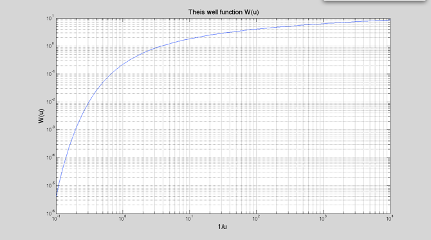
\includegraphics[width=0.8\textwidth]{pictures/2014_1}
\par\end{centering}
\caption{Theis well function type curve, ie, $\mathrm{W}\left(u\right)$ versus
$1/u$.}
\end{figure}


\section{Closed-book exam (1h), Feb 3, 2011}

\subsection{Question 1: Pressure in confined aquifer}

Question 1: Pressure in confined aquifer

A water level in a piezometer in a confined aquifer is affected if
the weight on a ground surface is suddenly changed. Compare two situations
a) Sudden change by a load placed on the ground, such as sand or flooding
by water and b) Sudden increase of the barometric pressure.

Case a: --- a load is placed on ground surface
\begin{enumerate}
\item How does the water pressure change in the piezometer? (Up? Down? Not?) 
\end{enumerate}
\rule[0.5ex]{1\columnwidth}{1pt}

Up

\rule[0.5ex]{1\columnwidth}{1pt}
\begin{enumerate}
\item How does the head change in the piezometer? (Up? Down? Not?) 
\end{enumerate}
\rule[0.5ex]{1\columnwidth}{1pt}

Up

\rule[0.5ex]{1\columnwidth}{1pt}

Case b: --- barometer pressure increased
\begin{enumerate}
\item How does the water pressure change in the piezometer? (Up? Down? Not? 
\end{enumerate}
\rule[0.5ex]{1\columnwidth}{1pt}

Up

\rule[0.5ex]{1\columnwidth}{1pt}
\begin{enumerate}
\item How does the head change in the piezometer? (Up? Down? Not?) 
\end{enumerate}
\rule[0.5ex]{1\columnwidth}{1pt}

Down

\rule[0.5ex]{1\columnwidth}{1pt}
\begin{enumerate}
\item If there is a difference between the two cases, then why is that? 
\end{enumerate}
\rule[0.5ex]{1\columnwidth}{1pt}

Although the water pressure in increased by the same amount in both
cases, the water level in the piezometer goes down in the case of
the increased barometric pressure, because the air pressure works
for 100\% on the water level inside the piezometer which is greater
than the increase of water pressure in the aquifer due to the air
pressure on ground surface. In the case of an increased load there
is no increase of pressure on the water level in the piezometer, and
so the change of water level in the piezometer fully reflects the
change of water pressure in the aquifer, which is some fraction of
the increase of pressure on ground surface.

\rule[0.5ex]{1\columnwidth}{1pt}

\subsection{Question 2: Tidal waves}

The groundwater head variation in a confined aquifer due to a tidal
wave at x=0 can be expressed mathematically as follows:

\[
s\left(x,t\right)=\phi\left(x,t\right)-\phi_{0}+A\,\exp\left(-ax\right)\sin\left(\omega t-ax\right)\mbox{, in which }a=\sqrt{\frac{\omega S}{2kD}}
\]

and $\omega=\frac{2\pi}{T}$ with $T$ the period of the wave.
\begin{enumerate}
\item What is the amplitude of the wave at distance $x$? 
\end{enumerate}
\rule[0.5ex]{1\columnwidth}{1pt}

\[
A_{x}=A_{0}\,e^{-ax}
\]

\rule[0.5ex]{1\columnwidth}{1pt}
\begin{enumerate}
\item What is the velocity of the wave? 
\end{enumerate}
\rule[0.5ex]{1\columnwidth}{1pt}

\[
\omega t-ax=\mathrm{const}=0\rightarrow v=\frac{x}{t}=\frac{\omega}{a}
\]

\rule[0.5ex]{1\columnwidth}{1pt}
\begin{enumerate}
\item If the wave would be just observable in a piezometer at x=1000 m from
the coast, then at what distance would the wave be just observable
on another spot along the coast where the storage coefficient is be
100 times greater than at the current spot and the transmissivity
is the same? 
\end{enumerate}
\rule[0.5ex]{1\columnwidth}{1pt}

So how to get the same amplitude at $x=0$ for both waves?

\[
A_{1}=A_{0}\,e^{-a_{1}L_{1}}=A_{0}\,e^{-a_{2}L_{2}}
\]

so

\[
a_{1}L_{1}=a_{2}L_{2}
\]

\[
\frac{\omega S_{1}}{2kD}L_{1}=\frac{\omega S_{2}}{2kD}L_{2}
\]

\[
S_{1}L_{1}=S_{2}L_{2}
\]

Therefore,

\[
L_{2}=L_{1}\frac{S_{1}}{S_{2}}=1000\times\frac{1}{100}=10\,\mathrm{m}
\]

\rule[0.5ex]{1\columnwidth}{1pt}
\begin{enumerate}
\item A tidal wave occurring daily is just observable in the aquifer at
a distance of x=500 m from shore. At what distance from the shore
will a 14-day wave be just observable occurring due to the monthly
moon cycle? Assume the same amplitude for both waves.
\end{enumerate}
\rule[0.5ex]{1\columnwidth}{1pt}

\[
\frac{\omega_{1}S}{2kD}L_{1}=\frac{\omega_{2}S}{2kD}L_{2}
\]

\[
\frac{\omega_{1}}{\omega_{2}}=\frac{L_{2}}{L_{1}}
\]

With $\omega_{1}=14\omega_{2}$ and $L_{1}=500\,\mathrm{m}$, we have
$L_{2}=14L_{1}=7000\,\mathrm{m}$.

\rule[0.5ex]{1\columnwidth}{1pt}

\subsection{Question 2: Characteristic time of groundwater systems}

In class we discussed the somewhat complicated solution by series
expansion of the evolution of the head after a sudden rain shower
of $P$ {[}m{]} in a strip of land of width $L$ {[}m{]} between parallel
fixed-head boundaries with water level $\phi_{0}$ {[}m{]}. We have
seen that after some time $t$ {[}d{]}, only the first term matters,
which is

\[
s\left(x,t\right)=\phi\left(x,t\right)-\phi_{0}=\frac{P}{S_{y}}\frac{4}{\pi}\cos\left(\pi\frac{x}{L}\right)\exp\left(-\pi^{2}\frac{kD}{L^{2}S_{y}}t\right)
\]

Whenever possible express your answers mathematically:
\begin{enumerate}
\item ~ What is the shape of the head?
\end{enumerate}
\rule[0.5ex]{1\columnwidth}{1pt}

A cosine

\rule[0.5ex]{1\columnwidth}{1pt}

What is the maximum head, take $\phi_{0}=0$?

\[
s\left(0,t\right)=\frac{P}{S_{y}}\frac{4}{\pi}\exp\left(-\pi^{2}\frac{kDt}{L^{2}S_{y}}\right)
\]

\begin{enumerate}
\item What would you consider the characteristic time of this system?
\end{enumerate}
\rule[0.5ex]{1\columnwidth}{1pt}

The most suitable definition may be this:

\[
T=\frac{L^{2}S}{\pi^{2}kD}
\]

Because it reduces the formula for the maximum head to:

\[
s\left(0,t\right)=\frac{P}{S_{y}}\frac{4}{\pi}\exp\left(-\frac{t}{T}\right)
\]

One could also choose another definition like

\[
T=\frac{L^{2}S}{4kD}=\frac{b^{2}S}{kD}
\]

Which may be better memorizable. It turn the formula into

\[
s\left(0,t\right)=\frac{P}{S_{y}}\frac{4}{\pi}\exp\left(-\frac{\pi^{2}}{4}\frac{t}{T}\right)
\]

\rule[0.5ex]{1\columnwidth}{1pt}
\begin{enumerate}
\item What would be the half-time of this groundwater system? 
\end{enumerate}
\rule[0.5ex]{1\columnwidth}{1pt}

The half-time is the time it takes for something to become half as
large. For exponential declining systems this is a constant. This
is the case here with the head relative to its final value. Let the
half-time be , then we can formally express the half-time as the time
it takes such that the ratio of the head at time is half the head
at time :

\[
\exp\left(-\xi\left(\frac{t+T_{50\%}}{T}\right)\right)=0.5\exp\left(-\xi\left(\frac{t}{T}\right)\right)
\]

\[
-\xi\left(t+T_{50\%}\right)=-T\ln2-\xi t
\]

\[
T_{50\%}=\frac{\ln2}{\xi}T
\]

where $\xi$ follows from the expression under the exponent, and threfore,
from the definition of the characteristic time.

\rule[0.5ex]{1\columnwidth}{1pt}

\subsection{Question 4: Wells}

The solution by Theis is given by

\[
s\left(r,t\right)=\phi_{0}-\phi\left(r,t\right)=\frac{Q_{0}}{4\pi kD}\mathrm{W}\left(u\right)\mbox{, where }u=\frac{r^{2}S}{4kDt}
\]

\begin{enumerate}
\item What flow conditions are described by Theis' well solution? 
\end{enumerate}
\rule[0.5ex]{1\columnwidth}{1pt}

The Theis solution describes the drawdown due to a well in a confined
(constant $kD$) aquifer extracting a flow $Q_{0}$\textsubscript{}
from $t=0$.

\rule[0.5ex]{1\columnwidth}{1pt}
\begin{enumerate}
\item What are its parameters and what are their dimensions? 
\end{enumerate}
\rule[0.5ex]{1\columnwidth}{1pt}
\begin{description}
\item [{$s$:}] {[}L{]} drawdown; {[}m{]} head relative to fixed datum
\item [{$Q_{0}$:}] {[}L\textsuperscript{3}/T{]} is the constant extraction
from the well.
\item [{$kD$:}] {[}L\textsuperscript{2}/T{]} aquifer transmissivity
\item [{$u$:}] {[}-{]} argument of well function
\item [{$r$:}] {[}m{]} distance from well
\item [{$S$:}] {[}-{]} storage coefficient of aquifer $S_{y}$\textsubscript{}or
$S_{S}D$
\item [{$t$:}] {[}T{]} time since the well started its extraction.
\end{description}
\rule[0.5ex]{1\columnwidth}{1pt}

As you know, the function W($u$) is the exponential integral, which
may be written as a series expansion :

\[
\mathrm{W}\left(u\right)=-0.577316-\ln u+u-\frac{u^{2}}{2\times2!}-\frac{u^{3}}{3\times3!}+\frac{u^{4}}{4\times4!}\cdots
\]

\begin{enumerate}
\item How can you mathematically approximate the Theis' solution for very
small values of $u$ given that $-0.577216\approx\ln\left(0.5615\right)$?
\end{enumerate}
\rule[0.5ex]{1\columnwidth}{1pt}

For sufficiently small $u$ we may truncate all terms above $\ln u$
in the series expression, to get

\[
\mathrm{W}\left(u\right)\approx-0.577361-\ln u\mbox{, where }u=\frac{r^{2}S}{4kDt}
\]

Fill in $u$ into the formula to obtain

\[
\mathrm{W}\left(u\right)\approx\frac{2.3Q}{4\pi kD}\log\left(\frac{2.25kDt}{r^{2}S}\right)
\]

\rule[0.5ex]{1\columnwidth}{1pt}
\begin{enumerate}
\item With this approximation, mathematically give the difference between
the drawdown obtained at time t and the drawdown at time 10t in a
piezometer at some arbitrary distance r from the well. 
\end{enumerate}
\rule[0.5ex]{1\columnwidth}{1pt}

\[
s_{10t}-s_{t}=\frac{2.3Q}{4\pi kD}\left[\log\left(\frac{2.25kD\left(10t\right)}{r^{2}S}\right)-\log\left(\frac{2.25kDt}{r^{2}S}\right)\right]=\frac{2.3Q}{4\pi kD}
\]

\rule[0.5ex]{1\columnwidth}{1pt}
\begin{enumerate}
\item Also give the difference between the drawdown in a piezometer at distance
r from the well and in a piezometer at distance 10r from the well,
both at the same time. 
\end{enumerate}
\[
s_{10t}-s_{t}=\frac{2.3Q}{4\pi kD}\left[\log\left(\frac{2.25kDt}{r^{2}S}\right)-\log\left(\frac{2.25kDt}{10^{2}r^{2}S}\right)\right]=\frac{2.3Q}{4\pi kD}\log\left(10^{2}\right)=\frac{2.3Q}{2\pi kD}
\]


\section{Closed-book exam (1h), Feb 5, 2010}

\subsection{Question 1:}
\begin{enumerate}
\item What is liquefaction? 
\end{enumerate}
\rule[0.5ex]{1\columnwidth}{1pt}

Loosely packed fine sand may become liquefied and turn into quicksand
by a shock (earthquake) by which grains become untached, the matrix
tries to resettle into a more compact configuration, but the water
cannot escape immediately due to the small conductivity of the fine
sand.

\rule[0.5ex]{1\columnwidth}{1pt}
\begin{enumerate}
\item What is the difference between specific yield and elastic storage? 
\end{enumerate}
\rule[0.5ex]{1\columnwidth}{1pt}

Water table storage versus storage due to the elastic properties of
both the water and the matrix.

\rule[0.5ex]{1\columnwidth}{1pt}
\begin{enumerate}
\item How does the specific yield change if an already shallow water table
rises? 
\end{enumerate}
\rule[0.5ex]{1\columnwidth}{1pt}

In a phreatic aquifer with a shallow water table, specific yield gets
smaller the shallower the water table. This is due to the moister
profile intersecting ground surface. See syllabus,

\rule[0.5ex]{1\columnwidth}{1pt}
\begin{enumerate}
\item Why does this happen (make a sketch and explain)?
\end{enumerate}
\rule[0.5ex]{1\columnwidth}{1pt}

See syllabus page 12.

\rule[0.5ex]{1\columnwidth}{1pt}
\begin{enumerate}
\item Which of the two materials, gravel and fine sand, has the highest
specific yield and why (assume both have the same porosity)? 
\end{enumerate}
\rule[0.5ex]{1\columnwidth}{1pt}

The coarser material has the highest specific yield because it has
the lowest specific retention, because less water can adhere against
gravity in the unsaturated zone because of the much smaller specific
surface in each volume of coarse material than the same volume of
fine material.

\rule[0.5ex]{1\columnwidth}{1pt}

\subsection{Question 2:}

The head in an aquifer connected to the ocean fluctuates due to tide.
This fluctuation is given by the following formula, in which \emph{s}
expresses the head variation caused by the tide as a function of time
\emph{t} and the inland distance from the shore \emph{x}:
\begin{quote}
\[
s\left(x,t\right)=A\,\exp\left(-ax\right)\sin\left(\omega t-ax\right)\mbox{, with }a=\sqrt{\frac{\omega S}{2kD}}
\]
\end{quote}
\begin{enumerate}
\item What is the expression for the maximum head fluctuation as a function
of \emph{x}? 
\end{enumerate}
This expression is just the part of the tide formula without the sine:

\rule[0.5ex]{1\columnwidth}{1pt}

\[
s\left(x,t\right)=A\,e^{-ax}
\]

\rule[0.5ex]{1\columnwidth}{1pt}
\begin{enumerate}
\item Sketch the head change s as a function of x at time t=0 and sketch
also the envelope (maximum and minimum value of s as a function of
x) 
\end{enumerate}
\begin{figure}
\begin{centering}
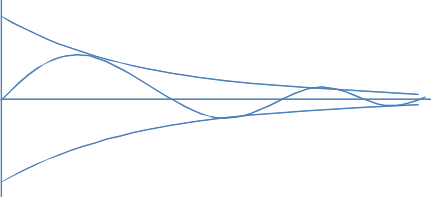
\includegraphics[width=0.8\textwidth]{pictures/2010_0}
\par\end{centering}
\caption{Sketch of wave as a function of $x$}

\end{figure}

\begin{enumerate}
\item Which parameters increase the inland penetration of the tide and which
parameters decrease this inland penetration? 
\end{enumerate}
\rule[0.5ex]{1\columnwidth}{1pt}

Parameters increasing the penetration depth of the tide wave are those
that reduce the value of the damping alfa, that is a lower frequency
omega, a lower storage coefficient and a higher transmissivity.

\rule[0.5ex]{1\columnwidth}{1pt}

\subsection{Question 3:}

Consider an extraction canal in direct contact with an aquifer of
infinite extent. The aquifer has transmissivity $kD=400\,\mathrm{m^{2}/d}$
and specific yield $S_{y}=0.1$. As long as $t<0$, the head in the
aquifer is everywhere 0 m (we take the initial water level as our
reference level).

At time $t=0\,\mathrm{d}$, the water level in the canal suddenly
changes to 2 m. Then, at time $t=2~\mathrm{d}$, the water level in
the canal suddenly changes back to its original value of 0 m and remains
constant afterwards.

The head change and the head-change gradient are:

\[
s=s_{0}\mathrm{erfc}\left(\sqrt{\frac{x^{2}S}{4kDt}}\right)\mbox{ and }\frac{\partial s}{\partial x}=-s_{0}\sqrt{\frac{S}{\pi kDt}}\exp\left(-\frac{x^{2}S}{4kDt}\right)
\]

To obtain values for the \textbf{$\mathrm{erfc}$ }function, use the
graph below.

Answer the following two questions.
\begin{enumerate}
\item Compute the head at $x=100\,\mathrm{m}$ at $t=3\,\mathrm{d}$. Show
the formula you use and include the dimension in your answer! 
\end{enumerate}
\rule[0.5ex]{1\columnwidth}{1pt}

This problem is solved by superposition in time:

\[
s=s_{0}\mathrm{erfc\left(\sqrt{\frac{x^{2}S}{4kDt}}\right)-s_{0}\mathrm{erfc}\left(\sqrt{\frac{x_{2}S}{4kD\left(t-3\right)}}\right)}
\]

Fill in the numbers to get your answer.

\rule[0.5ex]{1\columnwidth}{1pt}
\begin{enumerate}
\item Compute the discharge at $x=0$ at $t=3\,\mathrm{d}$. Show the formula
you use and include the dimension in your answer?
\end{enumerate}
\rule[0.5ex]{1\columnwidth}{1pt}

The discharge at x=0 as a function of time equals

\[
q\left(0,t\right)=-kD\frac{\partial s}{\partial x}=-kDs_{0}\sqrt{\frac{S}{\pi kDt}}
\]

so,

\[
q\left(0,3\right)=s_{0}\sqrt{\frac{kDS}{\pi}}\left(\sqrt{\frac{1}{t}}-\sqrt{\frac{1}{t-3}}\right)=2\sqrt{\frac{400\times0.1}{\pi}}\left(\sqrt{\frac{1}{3}}-\sqrt{\frac{1}{3-1}}\right)=-3.02\,\mathrm{m^{2}/d}
\]

\rule[0.5ex]{1\columnwidth}{1pt}

\begin{figure}
\begin{centering}
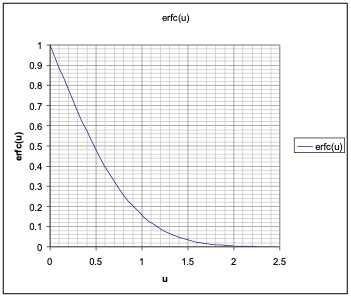
\includegraphics[width=0.7\textwidth]{pictures/2010_1}
\par\end{centering}
\caption{Function $\mathrm{erfc}\left(u\right)$}
\end{figure}


\subsection{Quesiton 4:}

Consider a well in a system of infinite extent which starts extracting
at time \emph{t}=0. We know that Theis' formula applies:

\[
s\left(r,t\right)=\frac{Q}{4\pi kD}\mathrm{W}\left(u\right)\mbox{, where }u=\frac{r^{2}S}{4kDt}
\]

We also know that for small values of \emph{u}, the well function,
W($u$), can be approximated by a straight line on log-t scale, which
is given by:

\[
\mathrm{W}\left(u\right)\approx2.3\log\left(\frac{0.5625}{u}\right)=2.3\log\left(\frac{2.25kDt}{r^{2}S}\right)
\]

Consider a pumping test on this well, starting the constant extraction
$Q=800\,\mathrm{m^{3}/d}$ at $t=0$. The drawdown is measured over
a number of days at an observation well at 25 m distance. The measured
drawdowns are shown in the figure below, which clearly reveals the
straight portion of the drawdown that we expect from the expression
above for large-enough values of time.
\begin{enumerate}
\item Using the straight line through the measured data, compute the transmissivity
\emph{$kD$} and the storage coefficient \emph{$S$} of this aquifer.
\end{enumerate}
\rule[0.5ex]{1\columnwidth}{1pt}

The drawdown difference per log cycle is the most convenient way to
compute the transmissivity. First draw a line through the straight
portion of the graph (see figure below) and then measure the drawdown
increase per log cycle, which is about 0.32 m. Then with log(10)=1,
compute the transmissivity from

\[
s_{10t}-s_{t}\approx\frac{2.3Q}{4\pi kD}\rightarrow kD=\frac{2.3Q}{4\pi\left(s_{10t}-s_{t}\right)}=\frac{1.3\times800}{4\pi0.32}\approx460\,\mathrm{m/d}
\]

Next we get the storage coefficient from the point where the straight
drawdown line of the above expression is zero, which is at about 0.12
days:

\[
\frac{2.25kDt}{r^{2}S}=1\rightarrow S=\frac{2.25kDt}{r^{2}}=\frac{2.25\times460\times0.12}{25^{2}}\approx0.2
\]

\rule[0.5ex]{1\columnwidth}{1pt}

\begin{figure}
\begin{centering}
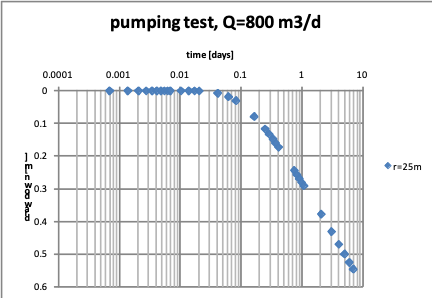
\includegraphics[width=0.8\textwidth]{pictures/2010_2}
\par\end{centering}
\caption{Measured drawdown during pumping test.}

\end{figure}


\section{Closed-book exam (3h), Feb 2009}

\subsection{Question 1:}
\begin{enumerate}
\item What is the difference between specific yield and elastic storage?
\end{enumerate}
\rule[0.5ex]{1\columnwidth}{1pt}

Storage coefficient in respectively unconfined and (semi)-confined
aquifers.

\rule[0.5ex]{1\columnwidth}{1pt}
\begin{enumerate}
\item How does the specific yield change if an already shallow water table
rises further and becomes even shallower? 
\end{enumerate}
\rule[0.5ex]{1\columnwidth}{1pt}

The specific yield becomes smaller.

\rule[0.5ex]{1\columnwidth}{1pt}
\begin{enumerate}
\item Why does this happen (make a sketch and explain)?
\end{enumerate}
\rule[0.5ex]{1\columnwidth}{1pt}

Part of the unsaturated profile that would store or yield water now
extends above ground surface, and no longer exists so that it cannot
contribute to storage.

\rule[0.5ex]{1\columnwidth}{1pt}
\begin{enumerate}
\item Which of the two materials, gravel and fine sand, has the highest
specific yield and why (assume both have the same porosity)? 
\end{enumerate}
\rule[0.5ex]{1\columnwidth}{1pt}

Fine sand, due to its much larger surface area and number contact
points between grains.

\rule[0.5ex]{1\columnwidth}{1pt}

\subsection{Question 2:}
\begin{enumerate}
\item What do we mean by Loading Efficiency ($LE$) and what do we mean
by Barometric Efficiency ($BE$)? 
\end{enumerate}
\rule[0.5ex]{1\columnwidth}{1pt}

$LE$ is the portion of the increased total pressure supported by
the water and increasing the head.

The $BE$ is the portion of the barometric pressure change causing
change of head.

Both $LE$ and $BE$ only work in (semi)-confined aquifers.

\rule[0.5ex]{1\columnwidth}{1pt}
\begin{enumerate}
\item What is the difference in terms of head change if we compare a loading
on land surface with an equal increase of the barometer pressure?
And why? 
\end{enumerate}
\rule[0.5ex]{1\columnwidth}{1pt}

In case of a load change, the head changes in the same direction ad
the load, with barometric change it changes in the opposite direction.
An increase of barometric pressure caused a decrease in head.

The difference is due to the face that the barometric pressure also
works in the piezometer, while a load increase does not.

\rule[0.5ex]{1\columnwidth}{1pt}

\subsection{Question 3:}

Tidal flow in a confined aquifer may be described mathematically by

\[
s=A\,e^{-ax}\sin\left(\omega t-ax\right)\mbox{, where }a=\sqrt{\frac{\omega S}{2kD}}
\]

\begin{enumerate}
\item What are the different quantities in these expressions and what are
their dimensions?
\end{enumerate}
\rule[0.5ex]{1\columnwidth}{1pt}
\begin{description}
\item [{$s$:}] head change due to the wave at $x=0$ {[}m{]}
\item [{\emph{$A$:}}] is amplitude of tide {[}m{]}
\item [{$a$:}] is dampoing factor {[}1/m{]}
\item [{$\omega$:}] is tidal frequency{[}radians/day{]}
\item [{\emph{$S$:}}] {[}-{]} is storage coefficient {[}-{]}
\item [{\emph{$kD$:}}] is transmissivity. {[}m$^{2}$/d{]}
\end{description}
\rule[0.5ex]{1\columnwidth}{1pt}
\begin{enumerate}
\item By what expression is the envelope given (the envelope describes the
maximum amplitude as a function of $x$?) 
\end{enumerate}
\rule[0.5ex]{1\columnwidth}{1pt}

\[
A_{x}=A_{0}\,e^{-ax}
\]

\rule[0.5ex]{1\columnwidth}{1pt}
\begin{enumerate}
\item How does the envelope change if the frequency of the tide would double? 
\end{enumerate}
It is reduced. Less penetration of the wave into the aquifer as follows
from.

\[
\frac{A_{x}}{A_{0}}=\exp\left(-\sqrt{\frac{\omega S}{2kD}}x\right)
\]

\begin{enumerate}
\item How will the envelope change if the transmissivity would be two times
less and the storage coefficient 100 times less? 
\end{enumerate}
The damping factor is

\[
a=\sqrt{\frac{\omega S}{2kD}}
\]

The larger $a$ the more damping and the less penetration of the wave
into the aquifer. A higher $\omega$ (frequency) increase the damping.
$\omega=0$ implies the lowest possible frequency, which yields no
damping, and, therefore the same $s$ independent of $x$, which is
equivalent to the steady stat situation. The damping is also increased
with higher $S$ and with lower $kD$.

\subsection{Question 4:}

The picture below shows a strip of land of width \emph{L} bounded
by two canals. Both the strip and the canals run perpendicular to
the paper (so the picture is a cross section). Suddenly the water
level in the left canal is raised by \emph{A} m as is indicated in
the figure. This causes the head to change in the strip. At the right
hand side the water level is unchanged. There exists an expression,
which mathematically describes the effect of a sudden level rise in
a strip that is unbounded on one side. We want to use this expression
to computed the head in the strip. We can do this by means of mirror
canals.

\begin{figure}
\begin{centering}
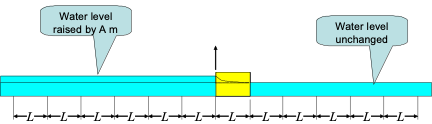
\includegraphics[width=1\textwidth]{pictures/2009_1}
\par\end{centering}
\caption{Strip of land of width \emph{L} bounded by open water. The water level
at the left hand side was suddenly raised by \emph{A} m. This causes
the head in the aquifer of the strip to change dynamically.}
\end{figure}

\begin{enumerate}
\item Irrespective of what the mathematical looks like, where would you
put the mirror canals and which are positive and which are negative?
Just draw an arrow respectively up or down (see figure) at the locations
where you would put the mirror canal.
\end{enumerate}
\begin{figure}
\begin{centering}
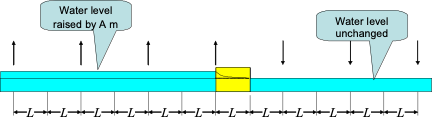
\includegraphics[width=1\textwidth]{pictures/2009_2}
\par\end{centering}
\caption{Same as previous figure, but now with superposition scheme shows by
the arrows.}
\end{figure}


\subsection{Question 5:}

The characteristic dynamics of a groundwater systems (i.e., the time
it takes for the head of a groundwater system to reach equilibrium)
is related to the argument of transient groundwater flow solutions,
This argument is $\sqrt{\frac{x^{2}S}{4kDt}}$ in solutions for one-dimensional
flow and $\frac{r^{2}S}{4kDt}$ for radial flow such as in the well
functions of Theis and Hantush.
\begin{enumerate}
\item Explain how the characteristic dynamics relate to these arguments? 
\end{enumerate}
\rule[0.5ex]{1\columnwidth}{1pt}

In a system of given width $L$ the factor $T=\frac{L^{2}S}{4kDt}$
has dimension time and is directly related to the dynamics of a groundwater
basin. It can be considered the characteristic time of the basin/system.

\rule[0.5ex]{1\columnwidth}{1pt}
\begin{enumerate}
\item Compare the characteristic dynamics of two systems. System two is
twice as wide as system one and its transmissivity is 3 times as large
and its storage coefficient 100 times as small as that of system one.
How do the dynamics of these two systems relate to each other, that
is: how many times faster or slower is system two compared to system
one in reaching piezometric equilibrium? 
\end{enumerate}
The factor $T=\frac{L^{2}S}{4kDt}$ with dimensions time is a measure
for the characteristic time of the groundwater system. System \#2
thus has a characteristic time that is $2^{2}\times0.01/3=0.013\approx1/75$
times larger or 75 times smaller than system \#1.

\subsection{Question 6:}

Consider a well in a semi-confined aquifer with $kD=900\,\mathrm{m^{2}/d}$,
$S=0.001$ and $c=400\,\mathrm{d}$ that is pumped at a discharge
$Q=2400\,\mathrm{m^{3}/d}$.
\begin{enumerate}
\item How long does it take before the drawdown at 60 m distance from the
well becomes stationary?
\end{enumerate}
\[
\lambda=\sqrt{kDc}=\sqrt{900\times400}=600\,\mathrm{m}\rightarrow\frac{r}{\lambda}=\frac{60}{600}=0.1
\]

See where the Hantush type curve for $r/\lambda=0.1$ becomes horizontal
(stationary). Read the $1/u$ value, which is about 1000, and compute
the time.

\[
\frac{1}{u}=\frac{4kDt}{r^{2}S}\rightarrow t=\frac{r^{2}S}{4kDu}=\frac{60^{2}\times0.001}{4\times900}\times1000\approx1.0\,\mathrm{d}
\]

\begin{enumerate}
\item What is the final drawdown? 
\end{enumerate}
This drawdown, because it is steady state can be computed either by
the De Glee formula (with the Bessel Function) or with the Hantush
formula

\[
s=\frac{Q}{2\pi kD}\mathrm{K_{0}}\text{\ensuremath{\left(\frac{r}{\lambda}\right)}=\ensuremath{\frac{Q}{4\pi kD}\mathrm{W}\left(u,\frac{r}{\lambda}\right)}}
\]

This is true, because the flow is steady state.

Using the type curves given we apply Hantush which yields with $1/u=100$0
and $r/L=0.1$, $\mathrm{W\left(\cdots\right)}=1.9$, so

\[
s=\frac{2400}{4\pi900}1.9\approx0.4\,\mathrm{m}
\]


\subsection{Quesiton 7:}

A pumping test has been carried out in a confined aquifer. The drawdown
and the Theis type curves are given in the graphs below. Theses graphs
have been drawn on the same type of double logarithmic paper. The
extraction of the well during the test was 1000 m\textsuperscript{3}/d.
Determine the transmissivity and the storage coefficient of this groundwater
system.

\begin{figure}
\begin{centering}
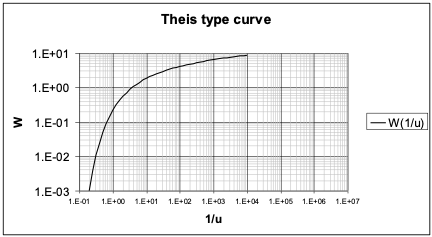
\includegraphics[width=0.8\textwidth]{pictures/2009_3}
\par\end{centering}
\caption{Theis well function Type curve.}
\end{figure}

\begin{figure}
\begin{centering}
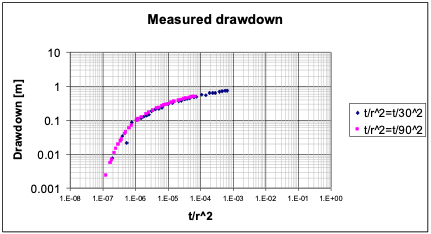
\includegraphics[width=0.8\textwidth]{pictures/2009_4}
\par\end{centering}
\caption{Measured drawdown versus $t/r^{2}.$}
\end{figure}

\begin{figure}
\begin{centering}
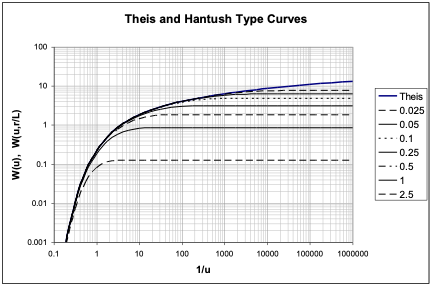
\includegraphics[width=0.8\textwidth]{pictures/2009_5}
\par\end{centering}
\caption{Theis and Hantush well function type curves.}
\end{figure}

\rule[0.5ex]{1\columnwidth}{1pt}

Fold the paper and tear off the lower graph. Shift the two graphs
over each other until they match (keep axes parallel). Then choose
a ``match point'' and read the combined value of $s$ and $\mathrm{W}$
to obtain $kD$ from

\[
s=\frac{Q}{4\pi kD}\mathrm{W\rightarrow kD=\frac{Q}{4\pi s}\mathrm{W}}
\]

With numbers read from both graphs once overlaid ($\mathrm{W}=1$
and $s=0.1\,\mathrm{m}$)

\[
kD=\frac{Q}{4\pi S}\mathrm{W}=\frac{1000}{4\pi0.1}\times1\approx795\,\mathrm{m/d}
\]

Then read the combined values of $1/u$ and $t/r^{2}$ from the graphs
and determine $S/kD$ from

\[
\frac{1}{u}=\frac{4kD}{S}\frac{t}{r^{2}}\rightarrow\frac{S}{kD}=4u\frac{t}{r^{2}}
\]

In numbers with $1/u\approx1.0$ and $t/r^{2}\approx3\times10^{-7}$
we get

\[
\frac{S}{kD}=4u\frac{t}{r^{2}}=4\times1\times3\times10^{-7}=1.2\times10^{-6}\,\mathrm{d/m^{2}}
\]

Finally compute $S=1.2\times10^{-6}\times kD=1.2\times10^{-6}\times795\approx10^{-3}$.

\rule[0.5ex]{1\columnwidth}{1pt}

\section{Closed-book exam (3h), Feb 2007}

\subsection{Question 1: Conceptual}
\begin{enumerate}
\item What is specific yield?
\end{enumerate}
\rule[0.5ex]{1\columnwidth}{1pt}

Specific yield, $S_{y}$, is the reversible storage caused by filling
and emptying of pores. Hence, it is the storage coeffiicent for the
phreatic or water-table aquifer.

\rule[0.5ex]{1\columnwidth}{1pt}
\begin{enumerate}
\item How does specific yield depend on the distance of the water table
below ground level? 
\end{enumerate}
\rule[0.5ex]{1\columnwidth}{1pt}

The shallower the water table above some depth, the lower the specific
yield. This is due to the moisture curve intersecting ground surface,
due to which the contents below the remaining moisture curve is less
than when it does not intersect ground surface.

\rule[0.5ex]{1\columnwidth}{1pt}
\begin{enumerate}
\item What happens to the water table in a piezometer in a confined aquifer
when the barometer pressure goes up, why? 
\end{enumerate}
\rule[0.5ex]{1\columnwidth}{1pt}

The water table goes down by the amount of the increased (changed)
barometer pressure (divided by $\rho g$ of course, to convert from
pressure to water column) that is not supported by the aquifer grain
matrix.

\rule[0.5ex]{1\columnwidth}{1pt}

\subsection{Question 2: Diffusion equation}

The diffusion equation for transient flow in one dimension is $D\frac{\partial^{2}s}{\partial x^{2}}=\frac{\partial s}{\partial t}$
\begin{enumerate}
\item What is the dimension of the diffusivity \emph{D}? 
\end{enumerate}
\rule[0.5ex]{1\columnwidth}{1pt}

It's always {[}L$^{2}$/T{]}. (This follows immediately from the partial
differential equation.)

\rule[0.5ex]{1\columnwidth}{1pt}
\begin{enumerate}
\item What is diffusivity \emph{D} in the case of groundwater flow? 
\end{enumerate}
\rule[0.5ex]{1\columnwidth}{1pt}

Ease of flow divided by storage, hence $kD/S$.

\rule[0.5ex]{1\columnwidth}{1pt}
\begin{enumerate}
\item What is diffusivity \emph{D} in the case of heat flow? 
\end{enumerate}
\rule[0.5ex]{1\columnwidth}{1pt}

Ease of flow divided by strorage, hence, $\frac{\lambda}{\rho c}$,
i.e., head conductance over specific head capacity

\[
\frac{\lambda}{\rho c}=\mathrm{[\frac{E}{TL^{2}}/(\frac{K}{L})]/[\frac{M}{L^{3}}\frac{E}{MK}]=[L^{2}/T],\,e.g.,\,m^{2}/s,\,mm^{2}/s\,etc}.
\]

\rule[0.5ex]{1\columnwidth}{1pt}

\subsection{Question 3: Fluctuation groundwater}

In the case of a tidal fluctuation in a river in direct contact with
an aquifer having transmissivity the fluctuation of the head may be
described by

\[
s=s_{0}\exp\left(-ax\right)\sin\left(\omega t-ax\right)\mbox{, with }a=\sqrt{\frac{\omega S}{2kD}}
\]

\begin{enumerate}
\item What is \emph{$s$} and what does this function look like? Make a
sketch of \emph{s} as a function of \emph{x}, and show its envelopes.
(The envelope is the curve of the values between which the function
fluctuates, as a function of $x$).
\end{enumerate}
\rule[0.5ex]{1\columnwidth}{1pt}

Lowercase \emph{$s$} {[}m{]} is the head change that is only due
to the wave (driven by the given fluctuation at $x=0$. The function
is a damped sine wave, i.e. it fluctuatuates between its envelopes
defined by $\pm A\exp(-ax)$.

\rule[0.5ex]{1\columnwidth}{1pt}
\begin{enumerate}
\item In the case of a double-day tide, $\omega=\frac{4\pi}{24}\,\mathrm{h^{-1}}$,
what would be the speed of the wave into the aquifer if $S=0.001$
and $kD=500\,\mathrm{m^{2}/d}$? (Notice the dimensions!) 
\end{enumerate}
\rule[0.5ex]{1\columnwidth}{1pt}

The speed of the wave follows from keeping the argument of the sine
constant. This leads to the expression $\omega t-ax=\mathrm{const}$.
To get the velocity, differentiate with respect to \emph{t} to get
$\omega-a\frac{dx}{dt}=0$, to $v=\frac{dx}{dt}=\frac{\omega}{a}$.
At what distance from the river is the amplitude of the head fluctuation
still only half of that in the river at $x=0$?

\rule[0.5ex]{1\columnwidth}{1pt}
\begin{enumerate}
\item What happens to this distance in case the transmissivity would be
9 times a big? 
\end{enumerate}
\rule[0.5ex]{1\columnwidth}{1pt}

Note that $a=\sqrt{\frac{\omega S}{2kD}}$. Hence a 9 times larger
$\text{\ensuremath{kD}}$ causes a 3 times lower value of the damping
factor `$a$` and so, a 3 times higher velocity of the wave.

\rule[0.5ex]{1\columnwidth}{1pt}

\subsection{Question 4: Flow to an extraction canal}

Consider an extraction canal in direct full contact with an aquifer
with transmissivity $kD=400\,\mathrm{m^{2}/d}$ and specific yield
$S_{y}=0.1$. The water level in the canal suddenly changes by 2 m
downward. The head and gradient are given by:

\[
s=s_{0}\mathrm{erfc}\left(\sqrt{\frac{x^{2}S}{4kDt}}\right)\mbox{ and }\frac{\partial s}{\partial x}=-s_{0}\sqrt{\frac{S}{\pi kDt}}\exp\left(-\frac{x^{2}S}{4kDt}\right)
\]

\begin{enumerate}
\item Compute the discharge into the canal after 1d. Show the formula you
use and include the dimension in your answer! 
\end{enumerate}
\rule[0.5ex]{1\columnwidth}{1pt}

Easy, just fill in the numbers.

\rule[0.5ex]{1\columnwidth}{1pt}
\begin{enumerate}
\item What is the head change \emph{$s$} at 100 m from the canal after
1 and after 2 d? (Use erfc-curve further down). 
\end{enumerate}
\rule[0.5ex]{1\columnwidth}{1pt}

Just fill in the numbers after reading the right values from the curve
of the erfc-function.

\rule[0.5ex]{1\columnwidth}{1pt}
\begin{enumerate}
\item What is the head change at 100 m from the canal after 2 days if the
head in the river would change back by 2 m at $t=1\,\mathrm{d}$? 
\end{enumerate}
\rule[0.5ex]{1\columnwidth}{1pt}

This requires superposition. Let the effect of the sudden head change
at t=0 continue forever and subtract the effect of the sudden head
change occurring at $t=2\,\mathrm{d}$ forever.

\rule[0.5ex]{1\columnwidth}{1pt}

\subsection{Question 5: Well in semi-confined aquifer}

Consider a transient well in a semi0-confined aquifer so that Hantush's
solution is valid, hence,

\[
s=\frac{Q}{4\pi kD}\mathrm{W}\left(u,\frac{r}{\lambda}\right)\mbox{, with }u=\frac{r^{2}S}{4kDt}\mbox{ and }\lambda=\sqrt{kDc}
\]

with $kD=600\,\mathrm{m^{3}/d}$, $c=900\,\mathrm{d}$, $S=0.001$
and pumping at a rate $Q=2400\,\mathrm{m^{3}/d}$.
\begin{enumerate}
\item How long does it take before steady state is reached for a point at
\emph{r}=300 m from the well (why)? Use Hantush type curves (see graphic
at the end of this exam). 
\end{enumerate}
\rule[0.5ex]{1\columnwidth}{1pt}

Compute $r\text{/}\lambda$ and look in the curve below when the line
for this value becomes horizontal, therefore, steady state. Use the
corresponding value of $1\text{/}u$ which is $4kDt\text{/}\left(r^{2}S\right)$,
fill in the know values of $\text{\ensuremath{kD}}$, $r$ and $S$
and compute the time $t$

\rule[0.5ex]{1\columnwidth}{1pt}

\subsection{Question 6: Drawdown due to a pumping station in an unconfined aquifer}

A well is situated at 100 m from an impermeable infinitely long wall.
The well is pumping at a rate of 2400 m\textsuperscript{3}/d. Even
though the aquifer is unconfined, the transmissivity \emph{$kD$}
may be taken as a constant equal to 600 m\textsuperscript{2}/d, while
the specific yield \emph{$S_{y}$}\textsubscript{} equals 0.2. The
well bore has a radius of $r_{0}=0.25\,\mathrm{m}$.
\begin{enumerate}
\item What is the drawdown at the well bore after 10 days of pumping ? 
\end{enumerate}
\rule[0.5ex]{1\columnwidth}{1pt}

The wall is impermeable, so we must place a mirror well with the same
pumping rate at 100 m beyond the wall to compute the drawdown. The
drawdown is then obtained by the superposition of the well and its
mirror well:

\[
s(0.25,t)=\frac{Q}{4\pi\text{kD}}\left(W_{h}\left(\frac{0.25^{2}S}{4\text{kDt}},\frac{0.25}{\lambda}\right)+W_{h}\left(\frac{200^{2}S}{4\text{kDt}},\frac{200}{\lambda}\right)\right)
\]

Just fill in the numbers for $\text{kD}$, $S$, $\lambda=\sqrt{\text{kDc}}$
and $t$=10 d, look up the value for $W_{h}\left(u,\frac{r}{\lambda}\right)$
in the graph and compute the answer.

\rule[0.5ex]{1\columnwidth}{1pt}
\begin{enumerate}
\item A well in a confined aquifer of infinite extent, with $kD=1000\,\mathrm{m^{2}/d}$
and $S=0.001$, is pumping at a rate of $Q=24000\,\mathrm{m^{3}/d}$.
How far would the radius of influence of this well after 100 years?
The radius of influence is the radius beyond which the drawdown is
considered negligible. You may exploit the logarithmic approximation
of the Theis well function for large times: 
\end{enumerate}
\[
\mathrm{W}\left(u\right)\approx\ln\left(\frac{0.5625}{u}\right)\mbox{, with }u<0.1\mbox{ and }u=\frac{r^{2}S}{4kDt}
\]

by making it zero.

The long-term drawdown in a confined aquifer due to a well pumping
from $t=0$ at a constant rate is given by the Theis equation, which
approaches a logarithmic function for large enough times (see given
formula of $\mathrm{W}(u)$). A practical approximation of the area
of influence is where this approximation of the Theis solution, hence,
the linear drawdown on half-log paper is zero. This is mathematically
done by setting the argument of the log equal to 1. Hence,

\[
\frac{0.5625}{u}=\frac{0.5625\times4kDt}{r^{2}S}=1\mbox{, and, therefore, }r=\sqrt{\frac{2.25kDt}{S}}
\]

\begin{figure}
\begin{centering}
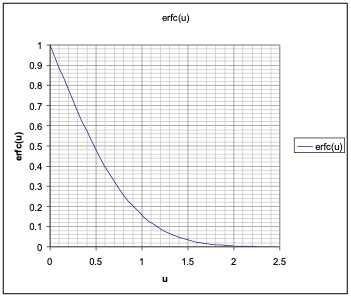
\includegraphics[width=0.8\textwidth]{pictures/2007_1}
\par\end{centering}
\caption{$\mathrm{erfc}\left(u\right)$function.}
\end{figure}

\begin{figure}
\begin{centering}
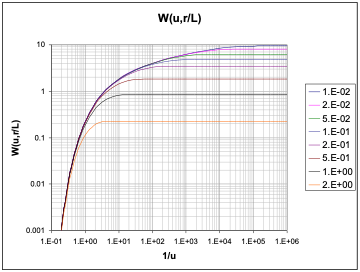
\includegraphics[width=0.8\textwidth]{pictures/2007_2}
\par\end{centering}
\caption{Theis and Hantush type curves. In case this graph is copied in black
and white only, note that the lowest type curve is for the highest
value of \emph{$r/\lambda$.} Note that the $L$ in the title and
left axis of this figure stands for $\lambda=\sqrt{kDc}$ value}
\end{figure}


\section{Closed-book exam (3h) Feb 2006}

\subsection{Question 1: Conceptual}
\begin{enumerate}
\item What types of reversible storage do you know in aquifer systems, explain
how it works 
\end{enumerate}
\rule[0.5ex]{1\columnwidth}{1pt}

Pore-water storage (by filling and emptying of pores) know as specific
yield, and elastic storage by compression and expansion of the aquifer
matrix and the water. Note that when the water pressure increases,
the pore matrix expands while the water is compressed.

\rule[0.5ex]{1\columnwidth}{1pt}
\begin{enumerate}
\item What values may you expect for the respective storage coefficients? 
\end{enumerate}
\rule[0.5ex]{1\columnwidth}{1pt}

Specific yield values will range between a few percent to around 25\%
depending on the pore space and for very fine pores also on the time
scale at which the head or water table varies. Elastic storage will
be in the order of 10e-3 depending on the natural stress of the aquifer
and its thickness, and the specific storage coefficient in the order
of 10e-5/m mainly depending on the natural stress on the grains.

\rule[0.5ex]{1\columnwidth}{1pt}
\begin{enumerate}
\item What is barometric efficiency, explain how it works. 
\end{enumerate}
\rule[0.5ex]{1\columnwidth}{1pt}

The barometric efficiency, $BE$, is the fraction of the barometer
pressure change that will cause drawdown in a (semi) confined aquifer.
The barometer pressure change is partly taken up by the aquifer matrix
(the loading efficiency $\text{\ensuremath{LE}}$) while the rest
of supported by a change in head (the barometric efficiency $\text{\ensuremath{BE}}$).
The essence is $BE+LE=1$.

\rule[0.5ex]{1\columnwidth}{1pt}
\begin{enumerate}
\item When the barometric pressure increases, does the head (water table
in a piezometer) in the confined aquifer rise or fall? 
\end{enumerate}
\rule[0.5ex]{1\columnwidth}{1pt}

It falls, because the water pressure in the aquifer increases by the
part not supported by the grains, i.e., by $\text{LE}\times p_{a}$
while the barometer pressure presses with full $p_{a}$ on the water
surface in the piezometer. Hence its level must decline by $p_{a}(1-LE)\text{/}(\rho g)$
to keep pressure equilibrium.

\rule[0.5ex]{1\columnwidth}{1pt}
\begin{enumerate}
\item Between what values may the barometric efficiency vary? 
\end{enumerate}
\rule[0.5ex]{1\columnwidth}{1pt}

Between 960 and 1040 hPa, or about 9.6 and 10.4 m water column.

\rule[0.5ex]{1\columnwidth}{1pt}
\begin{enumerate}
\item What happens in a confined aquifer with the head if a load is suddenly
placed on ground surface, such as a train stopping near a piezometer?
What happens when it leaves? Sketch a graph showing the head versus
time that you would expect in that case. 
\end{enumerate}
\rule[0.5ex]{1\columnwidth}{1pt}

The head increases initially with about $\text{\ensuremath{LE}\ }\Delta p$
where $\Delta p$ is the pressure increase in the aquifer due to the
train arriving. The pressure then drops off as the local head increase
below the train causes the groundwater to flow away so that after
a while the head is the same as before. The opposite happens when
the train leaves.

\rule[0.5ex]{1\columnwidth}{1pt}

\subsection{Question 2: Characteristic time of groundwater basin}

Characteristic time of groundwater basin, the partial differential
equation of which reads

\[
kD\frac{\partial^{2}\phi}{\partial x^{2}}=S\frac{\partial\phi}{\partial t}
\]

\begin{enumerate}
\item What is a characteristic time of a groundwater basin that may be considered
as one-dimensional of characteristic size \emph{L}? (hint: Make partial
differential equation dimensionless by setting $\xi=\frac{x}{L}$,
$\tau=\frac{t}{T}$ and see what $T$ is. 
\end{enumerate}
\rule[0.5ex]{1\columnwidth}{1pt}

The partial differential equation will then be converted into

\[
\frac{kD}{L^{2}}\frac{\partial\phi^{2}}{\partial\xi^{2}}=\frac{S}{T}\frac{\partial\phi}{\partial\tau}
\]

or

\[
\frac{\partial\phi^{2}}{\partial\xi^{2}}=\frac{L^{2}S}{\text{kDT}}\frac{\partial\phi}{\partial\tau}
\]

So that setting $\frac{L^{2}S}{kDT}=1$ gives that $T=\frac{L^{2}S}{kD}$
can be considered a characteristic time of the groundwater system
of size $L$ (with $L$ the approximate distance between opposite
head boundaries (distance between local reivers for instance).

\rule[0.5ex]{1\columnwidth}{1pt}
\begin{enumerate}
\item To reach equilibrium, how many times slower is a large basin compared
to a small one with the same transmissivity and storage coefficient? 
\end{enumerate}
\rule[0.5ex]{1\columnwidth}{1pt}

The size of the basin as measured by $L$ is squared in the characteristic
time. So, a basin where the $L$ is 5 times as large as another basin
is 25 times a slow in its drainage (natural drainage to equilibrium)

\rule[0.5ex]{1\columnwidth}{1pt}
\begin{enumerate}
\item Compute the characteristic time for the following cases:

\rule[0.5ex]{1\columnwidth}{1pt}

Large basin: \emph{kD}=500 m\textsuperscript{2}/d, system width \emph{L}=100km,
storage coefficient \emph{S}=0.2, 

\[
T=\frac{\left(10^{5}\right)^{2}\times0.2}{100}=2\times10^{7}\,d=\text{many},\text{many}\,\text{years}
\]

\rule[0.5ex]{1\columnwidth}{1pt}
\end{enumerate}
\rule[0.5ex]{1\columnwidth}{1pt}

Small basin: \emph{kD}=100 m\textsuperscript{2}/d, system width \emph{L}=100m
, storage coefficient \emph{S}=0.1 

\[
T=\frac{100^{2}\times0.1}{100}=10\,d
\]

\rule[0.5ex]{1\columnwidth}{1pt}

\subsection{Quesiton 3: Tides in groundwater}
\begin{quote}
Given: The tidal fluctuation in an aquifer in a point at distance
\emph{x} from the sea due to the water level fluctuation at sea with
amplitude \emph{A} is described by the following formula

\[
s\left(x,t\right)=A\,\exp\left(-ax\right)\sin\left(\omega t-ax\right)
\]

in which the damping factor is as follows $a=\sqrt{\frac{\omega S}{2kD}}$,
where $\omega$ is the angle velocity in radians/time or $\omega=\frac{2\pi}{T}$
where $T$ is the time of a complete wave cycle. 
\end{quote}
Are the following expressions true or false?
\begin{enumerate}
\item The wave in the aquifer has a different frequency than the tide itself.
\end{enumerate}
\rule[0.5ex]{1\columnwidth}{1pt}

False, it's physically unimaginable that the frequencies would be
different.

\rule[0.5ex]{1\columnwidth}{1pt}
\begin{enumerate}
\item The amplitude of the wave at a given distance from the sea becomes
greater when
\end{enumerate}
\rule[0.5ex]{1\columnwidth}{1pt}

The frequency of the tide is reduced?

The higher the frequency, so the higher $\omega$, to higher the damping
$a$ and, therefore, the smaller the distance over which the fluctuation
in the

aquifer can be felt. Only an infinitely slow frequency reaches to
infinity, as this is equivalent to the steady-state situation.

\rule[0.5ex]{1\columnwidth}{1pt}

The storage coefficient is reduced?

The smaller the storage coefficient the faster and the farther the
fluctuation travels inland. With a (theoretically) zero storage coefficient,
the wave would (only theoretically) travel with infinite speed, which
would imply that only a steady state situation would be possible (zero
storage) or that the head at all $x$ would be the same as at $x=0$.

\rule[0.5ex]{1\columnwidth}{1pt}

Then the transmissivity is reduced?

The transmissivity determines ease of flow. Hence if reduces flow
will be less easy. With zero transmissivity the fluctuation at zero
would not penetrate the aquifer at all, speed zero; on the other hand,
with transmissivity infinite, the speed of the wave would also be
(theoretically) infinite and yield the same result as storage coefficient
equal to zero.

\rule[0.5ex]{1\columnwidth}{1pt}

\subsection{Question 4: Aquifer with river}

Consider an aquifer of infinite extent bounded by a fully penetrating
river at $x=0$. At $t=0$ the river level suddenly changes by a height
$A$. The change of head $s(x,t)$ in the aquifer equals in this case:

\[
s\left(x,t\right)=A\,\mathrm{erfc}\left(\sqrt{\frac{x^{2}S}{4kDt}}\right)
\]

with $\mathrm{erfc}(u)$ as shown in the picture below

\begin{figure}
\begin{centering}
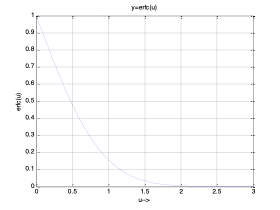
\includegraphics[width=0.8\textwidth]{pictures/2006_1}
\par\end{centering}
\caption{$\mathrm{erfc\left(u\right)}$versus $u$}
\end{figure}

\begin{enumerate}
\item What is the final value of the head change (the value reached after
infinite time, $s\left(x,\infty\right)$? 
\end{enumerate}
\rule[0.5ex]{1\columnwidth}{1pt}

That's simple: it must be A, the new steady level of the river.

\rule[0.5ex]{1\columnwidth}{1pt}
\begin{enumerate}
\item What value has the argument of $\mathrm{erfc}(\cdots)$, i.e., $\sqrt{\frac{x^{2}S}{4kDt}}$
when the head change is half the final value? 
\end{enumerate}
\rule[0.5ex]{1\columnwidth}{1pt}

From the graph it's seen that it's a fraction less than 0.5.

\rule[0.5ex]{1\columnwidth}{1pt}
\begin{enumerate}
\item If $kD=400\,\mathrm{m^{2}/d}$, $S=0.1$ and $x=100\,\mathrm{m}$,
after how much time is this the change of head equal to $0.5A$? 
\end{enumerate}
\rule[0.5ex]{1\columnwidth}{1pt}

This implies that the argument must be about 0.5, i.e.

\[
\frac{x^{2}S}{4\text{kDt}}=0.25
\]

Just fill in $\text{\ensuremath{kD}}$ and $S$ and compute $t$.

\rule[0.5ex]{1\columnwidth}{1pt}
\begin{enumerate}
\item What would be the formula if the head change occurred on time \emph{$t_{1}$}\textsubscript{}
instead of time$t=0$? 
\end{enumerate}
\rule[0.5ex]{1\columnwidth}{1pt}

\[
s(x,t)=A\ \text{erfc}\left(\frac{x^{2}S}{4\text{kD}\left(t-t_{1}\right)}\right)\mbox{, where }t>t_{1}
\]

Again, set the argument equal to 0.5 to compute t at which the drawdown
at $x$ is equal to $0.5\ A$.

\rule[0.5ex]{1\columnwidth}{1pt}
\begin{enumerate}
\item How could you compute the head change at point \emph{x} if the there
was a sudden change of the river level of \emph{A}\textsubscript{1}
at time \emph{t}=\emph{t}\textsubscript{1} and another of \emph{A}\textsubscript{2}
at \emph{t}=\emph{t}\textsubscript{2}? 
\end{enumerate}
\rule[0.5ex]{1\columnwidth}{1pt}

By superposition, in this case

\[
s(r,t)=A_{1}\text{erfc}\left(\frac{x^{2}S}{4\text{kD}\left(t-t_{1}\right)}\right)+A_{2}\text{erfc}\left(\frac{x^{2}S}{4\text{kD}\left(t-t_{2}\right)}\right)
\]

\rule[0.5ex]{1\columnwidth}{1pt}

\subsection{Question 5: Well in a confined aquifer}

Consider a well in a confined aquifer starting an extraction of $Q=1200\,\mathrm{m^{3}/d}$
at $t=0$. $kD=1000\,\mathrm{m^{2}/d}$, and $S=0.001$. For this
case the Theis solution applies:

\[
s=\frac{Q}{4\pi kD}\mathrm{W\left(u\right)\mbox{, with }}u=\frac{r^{2}S}{4kDt}
\]

(See the type curve of Theis well function on a separate page).
\begin{enumerate}
\item Compute the head at $r=20\,\mathrm{m}$ after $t=1\,\mathrm{d}$. 
\end{enumerate}
\rule[0.5ex]{1\columnwidth}{1pt}

\[
s(20,1)=\frac{1200}{4\pi1000}\mathrm{W}\left(\frac{20^{2}\times0.001}{4\times1000\times1}\right)
\]

Where the argument of $\mathrm{W}$ is $u$ for which $\mathrm{W}$
can be looked up in the type curve below.

\rule[0.5ex]{1\columnwidth}{1pt}
\begin{enumerate}
\item The pump is switched off after 1 day. What is the head after 1.1 days
at $r=20\,\mathrm{m}$? 
\end{enumerate}
\rule[0.5ex]{1\columnwidth}{1pt}

In that case we apply superposition. That is, we place another well
at the same spot and switch it on with $-Q$ at $t=1.1$ days and
add the two wells. In math:

\[
s(20,1.1)=\frac{Q}{4\pi kD}\left(\mathrm{W}\left(\frac{20^{2}S}{4kD\times1.1}\right)-\mathrm{W}\left(\frac{20^{2}S}{4kD\times(1.1-1.0)}\right)\right)
\]

Where the first term requires $t>0$ and the second $t>1.0$ d.

\rule[0.5ex]{1\columnwidth}{1pt}

\subsection{Question 6: Well in a leaky aquifer}

Consider a transient well in a leaky aquifer. $kD=400\,\mathrm{m^{2}/d}$,
$c=400\,\mathrm{d}$, $S=0.001$, so that the groundwater behaves
according to Hantush's transient well formula

\[
s=\frac{Q}{4\pi kD}\mathrm{W}\left(u,\frac{r}{\lambda}\right)\mbox{, with }\lambda=\sqrt{kDc}
\]

\begin{enumerate}
\item How long does it take until the head at $r=40\,\mathrm{m}$ becomes
steady state or virtually steady state? (Hint: look at the type curves
to get u for which this is the case, note). 
\end{enumerate}
\rule[0.5ex]{1\columnwidth}{1pt}

Compute $\frac{r}{\lambda}=\frac{40}{\sqrt{kDc}}$ and look for the
corresponding type curve in the graph with the type curves for the
Hantush well function. Look for which value of $1/u$ the curve becomes
horizontal, take the value of $1/u$ for the point, compute u and
apply this value in the formula for $u$, from which the time follows.

\rule[0.5ex]{1\columnwidth}{1pt}

\subsection{Question 7: Well in an unconfined aquifer}

Consider a well in an unconfined aquifer for which the Theis-solution
applies (see type curve hereafter. Further given a pumping test with
an extraction of $Q=600\,\mathrm{m^{3}/d}$ during which drawdown
measurements were made (see the graph with the small circles).

Interpret the test (that is: compute \emph{kD} and \emph{S}).

(Hint: if you can't see through the paper make the type curve thicker
using a pen and hold both curves up against a light or in the direction
of a window).

\rule[0.5ex]{1\columnwidth}{1pt}

Shift the curves on top of each other keeping the axes parallel until
you obtain the best possible fit. Then for that chosen (by arbitrary
point) read the corresponding values of $1/u$ and $1\text{/}r^{2}$
and of the drawdown $s$ and $\mathrm{W}(u)$.

The from the formula for the drawdown

$s=\frac{Q}{2\pi kD}\mathrm{W}(u)$ with now a corresponding value
of $s$ and $\mathrm{W}(u)$ known as well as $Q$ known, compute
the transmissivity. Next, with a corresponding value for $t\text{/}r^{2}$
and $1/u$ known and $kD$ just compute we have $\frac{4kD}{S}\frac{t}{r^{2}}=\frac{1}{u}$
from which the storage coefficient, $S$, follows. In the case of
a semi-confined aquifer, the match by shifting the graphs should also
provide the curve with a specific value of $r\text{/}\lambda$ that
best fits the measurements. This implies that with r known and $kD$
just determined we now also get the resistance c from $\lambda=\sqrt{kDc}$.

\rule[0.5ex]{1\columnwidth}{1pt}

\begin{figure}
\begin{centering}
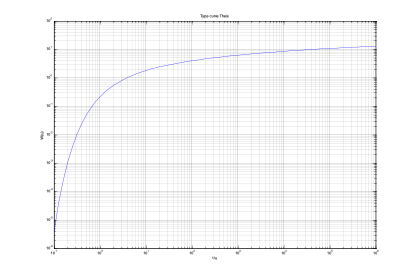
\includegraphics[width=0.8\textwidth]{pictures/2006_2}
\par\end{centering}
\caption{Theis type curve, $\mathrm{W}\left(u\right)$ versus $1/u$}
\end{figure}

\begin{figure}
\begin{centering}
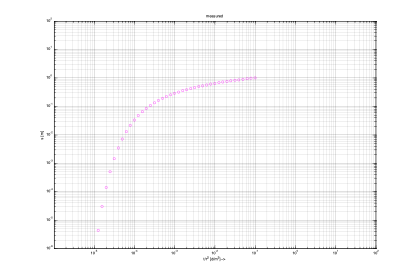
\includegraphics[width=0.8\textwidth]{pictures/2006_3}
\par\end{centering}
\caption{Measured drawdown during pumping test versus \emph{$t/r^{2}$})}
\end{figure}

\begin{figure}
\begin{centering}
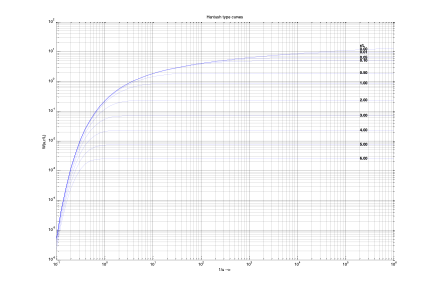
\includegraphics[width=0.8\textwidth]{pictures/2006_4}
\par\end{centering}
\caption{Theis and Hantush type curves combined, i.e., $\mathrm{W}\left(u\right)$
and $\mathrm{W}\left(u,\frac{r}{\lambda}\right)$ vs $1/u$.}
\end{figure}

\end{document}
